\documentclass[11pt,aspectratio=169]{beamer}

% ---------------------------------------------------------------
% Packages
% ---------------------------------------------------------------
\usepackage[utf8]{inputenc}
\usepackage[T1]{fontenc}
\usepackage[french]{babel}
\usepackage{lmodern}
\usepackage{graphicx}
\graphicspath{{figures/}{rapport/figures/}}
\PassOptionsToPackage{dvipsnames}{xcolor}
\usepackage{xcolor}
\usepackage{colortbl}
\definecolor{gold}{RGB}{218,165,32}
\usepackage{booktabs}
\usepackage{array}
\usepackage{tabularx}
\usepackage{amsmath,amssymb}
\usepackage{tikz}
\usetikzlibrary{shapes,arrows,positioning,fit,backgrounds,arrows.meta,calc}

% ---------------------------------------------------------------
% Thème Beamer
% ---------------------------------------------------------------
\usetheme{Madrid}
\usecolortheme{seahorse}
\useinnertheme{rectangles}
\useoutertheme{infolines}

\definecolor{enseirbblue}{RGB}{0,76,153}
\definecolor{enseirbaccent}{RGB}{200,80,40}
\definecolor{bidgreen}{RGB}{40,160,80}
\definecolor{askred}{RGB}{200,60,50}
\setbeamercolor{structure}{fg=enseirbblue}
\setbeamercolor{title}{fg=white,bg=enseirbblue}
\setbeamercolor{frametitle}{fg=white,bg=enseirbblue}
\setbeamercolor{block title}{fg=white,bg=enseirbblue}
\setbeamercolor{block body}{bg=enseirbblue!10}
\setbeamercolor{alerted text}{fg=enseirbaccent}

\setbeamertemplate{navigation symbols}{}
\setbeamertemplate{itemize item}{\color{enseirbblue}\textbullet}
\setbeamertemplate{itemize subitem}{\color{enseirbblue}--}

% ---------------------------------------------------------------
% Page de titre
% ---------------------------------------------------------------
\title[Order Book Engine]{Order Book Engine}
\subtitle{Carnet d'ordres haute performance \& agents de trading par RL}
\author[Équipe PFA]{Équipe PFA -- 6 membres}
\institute[ENSEIRB-MATMECA]{ENSEIRB-MATMECA \\ Projet de Fin d'Année}
\date{\today}

% ===============================================================
\begin{document}
% ===============================================================

% --- Slide 1 : Titre
\begin{frame}
    \titlepage
\end{frame}

% --- Slide 2 : Plan (visuel et compact)
\begin{frame}{Plan}
    \begin{columns}[T]
        \column{0.5\textwidth}
        \textbf{\color{enseirbblue}Infrastructure}
        \begin{enumerate}
            \item Contexte \& objectifs
            \item Architecture
            \item Moteur C++
            \item Données Binance
        \end{enumerate}
        \column{0.5\textwidth}
        \textbf{\color{enseirbblue}Stratégies}
        \begin{enumerate}\setcounter{enumi}{4}
            \item Stratégies par règles
            \item Dashboard
            \item Agents RL (DQN, A2C, PPO)
            \item Dreamer v3
            \item Résultats \& conclusion
        \end{enumerate}
    \end{columns}
\end{frame}

% ===============================================================
% PARTIE 1 -- Contexte
% ===============================================================

% --- Slide 3 : Contexte
\begin{frame}{Le défi des marchés modernes}
    \begin{columns}[c]
        \column{0.55\textwidth}
        \begin{itemize}
            \item \alert{$10^5$ ordres/s}
            \item Latence \alert{$\sim$ microseconde}
            \item Données \alert{temps réel}
        \end{itemize}
        \vspace{0.3cm}
        \begin{block}{Notre projet}
            Une plateforme \textbf{de bout en bout} pour simuler, entraîner et évaluer des stratégies sur données crypto.
        \end{block}

        \column{0.4\textwidth}
        \centering
        
\includegraphics[width=0.55\textwidth]{binance_logo.png}\\[0.4cm]
        \footnotesize Données live : Binance API
    \end{columns}
\end{frame}

% --- Slide 4 : Cahier des charges
\begin{frame}{Cahier des charges}
    \begin{center}
    \footnotesize
    \begin{tabular}{p{2.2cm}p{6cm}p{3.5cm}}
        \toprule
        \textbf{Type} & \textbf{Exigence} & \textbf{Concrètement} \\
        \midrule
        \rowcolor{enseirbblue!10}
        Fonctionnel & Matching prix-temps, 5 types d'ordres   & GTC, Market, IOC, FOK, GFD \\
        Fonctionnel & Ingestion de données réelles            & API Binance \\
        Fonctionnel & Agents enfichables + visualisation      & Dashboard web \\
        \rowcolor{enseirbblue!10}
        Non-fct.    & Performance haut débit                  & $\geq 10^5$ ops/s \\
        Non-fct.    & Latence opérationnelle                  & $\sim$ microseconde \\
        Non-fct.    & Reproductibilité                        & Seeds, checkpoints \\
        \bottomrule
    \end{tabular}
    \end{center}

    \vspace{0.4cm}
    \begin{center}
    \alert{\textbf{Hors périmètre :}} trading réel, conformité, FPGA.
    \end{center}
\end{frame}

% ===============================================================
% PARTIE 2 -- Architecture
% ===============================================================

% --- Slide 5 : Architecture logicielle
\begin{frame}{Architecture logicielle}
    \centering
    \begin{tikzpicture}[
        node distance=0.4cm and 0.7cm,
        every node/.style={font=\footnotesize},
        box/.style={draw, rounded corners, minimum width=2.4cm, minimum height=0.9cm, align=center},
        cppbox/.style={box, fill=enseirbblue!25},
        pybox/.style={box, fill=enseirbaccent!20},
        databox/.style={box, fill=gray!20},
        arr/.style={->, thick, >=stealth}
    ]
        \node[databox] (binance) {\textbf{Binance API} \\ \tiny REST};
        \node[cppbox, right=of binance] (live) {\textbf{LiveMarketData} \\ \tiny libcurl + JSON};
        \node[cppbox, right=of live]    (engine) {\textbf{Moteur C++} \\ \tiny matching};

        \node[databox, below=of live]   (jsonm) {\texttt{market\_state.json}};
        \node[databox, below=of engine] (jsono) {\texttt{agent\_orders.json}};

        \node[pybox, below=of jsonm] (agent) {\textbf{Agent Python}};
        \node[pybox, below=of jsono] (rl)    {\textbf{RL / Dreamer}};
        \node[pybox, left=of agent]  (dash)  {\textbf{Dashboard}};

        \draw[arr] (binance) -- (live);
        \draw[arr] (live) -- (engine);
        \draw[arr] (engine) -- (jsonm);
        \draw[arr] (jsonm) -- (agent);
        \draw[arr] (agent) -- (rl);
        \draw[arr] (rl) -- (jsono);
        \draw[arr] (jsono) -- (engine);
        \draw[arr] (jsonm) -- (dash);
    \end{tikzpicture}

    \vspace{0.3cm}
    \alert{Découplage par fichiers JSON} : composants C++ et Python relancés indépendamment.
\end{frame}

% ===============================================================
% PARTIE 3 -- Moteur C++
% ===============================================================

% --- Slide 6 : Carnet d'ordres (visualisation)
\begin{frame}{Carnet d'ordres}
    \centering
    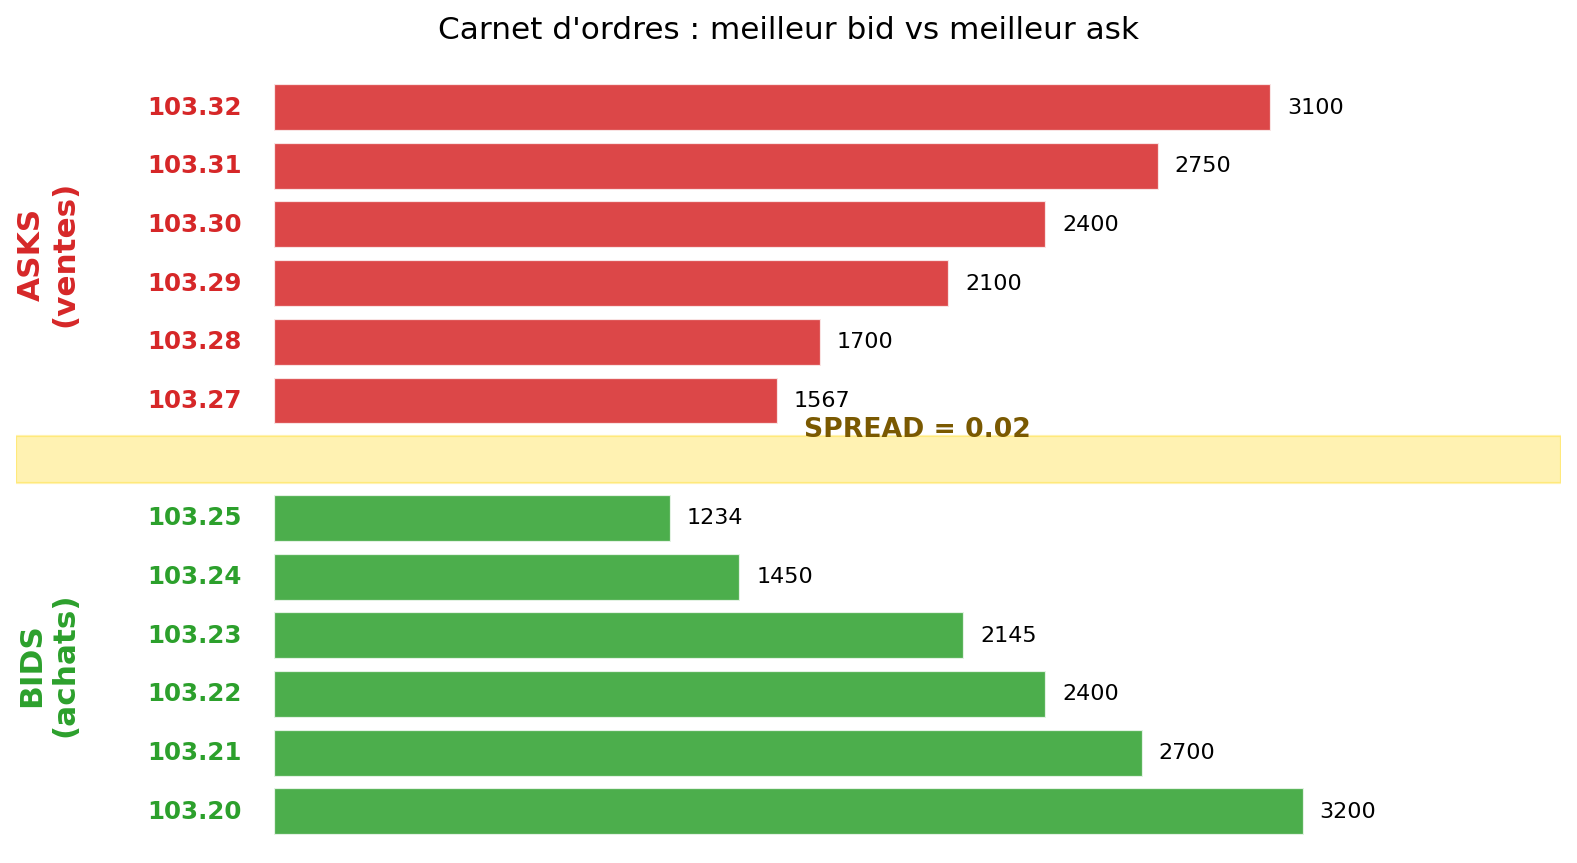
\includegraphics[width=0.78\textwidth]{orderbook_viz.png}

    \vspace{-0.2cm}
    \footnotesize
    Bids = ordres d'achat (prix décroissants) \quad $|$ \quad Asks = ordres de vente (prix croissants)
\end{frame}

% --- Slide 7 : Algorithme de matching
\begin{frame}{Matching prix-temps}
    \begin{columns}[c]
        \column{0.55\textwidth}
        \centering
        \begin{tikzpicture}[
            every node/.style={font=\footnotesize},
            buy/.style={draw=bidgreen, fill=bidgreen!15, rounded corners, minimum width=1.3cm, minimum height=0.6cm},
            sell/.style={draw=askred, fill=askred!15, rounded corners, minimum width=1.3cm, minimum height=0.6cm}
        ]
            % Buy side
            \node[buy] (b1) at (0,2.4) {\tiny 100 @ 103.25};
            \node[buy] (b2) at (0,1.7) {\tiny 200 @ 103.24};
            \node[buy] (b3) at (0,1.0) {\tiny 150 @ 103.23};

            % Sell side
            \node[sell] (s1) at (3,2.4) {\tiny 80 @ 103.27};
            \node[sell] (s2) at (3,1.7) {\tiny 200 @ 103.28};
            \node[sell] (s3) at (3,1.0) {\tiny 150 @ 103.29};

            \node at (0,3.05)   {\textbf{\color{bidgreen}BIDS}};
            \node at (3,3.05)   {\textbf{\color{askred}ASKS}};

            % Spread arrow
            \draw[<->, thick, gold!80!black] (0.7,2.4) -- (2.3,2.4);
            \node[fill=yellow!50, font=\tiny] at (1.5,2.4) {spread};

            % match arrow
            \node[draw=enseirbaccent, thick, fill=enseirbaccent!10, rounded corners, minimum width=4.5cm, minimum height=0.6cm] (match) at (1.5,0) {\textbf{Nouveau BUY 50 @ 103.27}};
            \draw[->, thick, enseirbaccent] (match) to[bend right=20] (s1);
            \node[font=\scriptsize, enseirbaccent] at (3.7,0.5) {match!};
        \end{tikzpicture}

        \column{0.42\textwidth}
        \begin{block}{Règles}
            \begin{enumerate}
                \item \alert{Meilleur prix} d'abord
                \item À prix égal : \alert{FIFO}
                \item Exécutions partielles permises
            \end{enumerate}
        \end{block}
        \vspace{0.2cm}
        \footnotesize
        Match dès que :
        \[
        P_{\text{buy}} \geq P_{\text{ask}}
        \]
    \end{columns}
\end{frame}

% --- Slide 8 : Structures de données et complexité
\begin{frame}{Structures de données}
    \begin{columns}[T]
        \column{0.5\textwidth}
        \footnotesize
        \begin{itemize}
            \item Deux \texttt{std::map} séparées (bids \alert{$\downarrow$}, asks \alert{$\uparrow$})
            \item Niveau de prix : \texttt{std::list} (FIFO)
            \item \texttt{unordered\_map<id, iter>} : annulation \alert{$O(1)$}
        \end{itemize}

        \column{0.5\textwidth}
        \scriptsize
        \begin{tabular}{lll}
            \toprule
            \textbf{Op.} & \textbf{Complexité} & \textbf{Débit} \\
            \midrule
            Ajout         & $O(\log n)$  & $\approx 400$\,k/s \\
            Annulation    & $O(1)$       & $\approx 2$\,M/s \\
            Modification  & $O(\log n)$  & $\approx 270$\,k/s \\
            Matching      & $O(k\log n)$ & $\approx 350$\,k/s \\
            \bottomrule
        \end{tabular}
    \end{columns}

    \vspace{0.3cm}
    \begin{block}{Performances mesurées}
        Latence \alert{2--4\,$\mu$s} sur matériel de développement standard.\\
        Cible $\geq 10^5$ ops/s : \textbf{atteinte}.
    \end{block}
\end{frame}

% --- Slide 9 : Types d'ordres
\begin{frame}{Cinq types d'ordres}
    \centering
    \begin{tikzpicture}[
        every node/.style={font=\footnotesize},
        type/.style={draw, rounded corners, fill=enseirbblue!15,
                     minimum width=2.5cm, minimum height=1.4cm, align=center}
    ]
        \node[type] (gtc) at (0,0) {\textbf{GoodTillCancel} \\ \tiny actif jusqu'à \\ \tiny annulation};
        \node[type] (mkt) at (3,0) {\textbf{Market} \\ \tiny limit \\ \tiny agressif};
        \node[type] (ioc) at (6,0) {\textbf{IOC} \\ \tiny exéc. partielle, \\ \tiny reste annulé};
        \node[type] (fok) at (9,0) {\textbf{FillOrKill} \\ \tiny tout ou \\ \tiny rien};
        \node[type] (gfd) at (12,0) {\textbf{GoodForDay} \\ \tiny expire \\ \tiny à 15:59};
    \end{tikzpicture}

    \vspace{0.6cm}
    \begin{block}{Tests fonctionnels}
        Suite \texttt{OrderBookTests} couvre les 5 types : insertion, annulation, modification, exécution partielle, rejet \texttt{FillOrKill}, expiration \texttt{GFD}.
    \end{block}
\end{frame}

% ===============================================================
% PARTIE 4 -- Données + règles + dashboard
% ===============================================================

% --- Slide 10 : Pipeline Binance
\begin{frame}{Pipeline d'ingestion temps réel}
    \centering
    \begin{tikzpicture}[
        node distance=1cm,
        every node/.style={font=\footnotesize},
        box/.style={draw, rounded corners, minimum width=2.4cm, minimum height=1cm, align=center},
        arr/.style={->, very thick, >=stealth, enseirbblue}
    ]
        \node[box, fill=yellow!20] (api) {\textbf{Binance API}\\\tiny REST/JSON};
        \node[box, right=of api, fill=enseirbblue!20]  (curl) {\textbf{libcurl}\\\tiny HTTP};
        \node[box, right=of curl, fill=enseirbblue!20] (parse){\textbf{nlohmann/json}\\\tiny parsing};
        \node[box, right=of parse, fill=enseirbblue!25](book) {\textbf{Order Book}\\\tiny C++};
        \node[box, below=of book, fill=gray!15]        (json) {\texttt{market\_state}\\\tiny JSON};

        \draw[arr] (api) -- (curl);
        \draw[arr] (curl) -- (parse);
        \draw[arr] (parse) -- (book);
        \draw[arr] (book) -- (json);
    \end{tikzpicture}

    \vspace{0.4cm}
    \begin{columns}[T]
        \column{0.5\textwidth}
        \textbf{Lancement}
        \begin{block}{}
            \texttt{./LiveMarketData SOLUSDT 1 20}
        \end{block}
        \column{0.5\textwidth}
        \textbf{Sorties live}
        \begin{itemize}
            \item Bid / Ask / Mid / Spread
            \item Profondeur, SMA, PnL
        \end{itemize}
    \end{columns}
\end{frame}

% --- Slide 11 : Mean Reversion (visuel)
\begin{frame}{Stratégie : Mean Reversion}
    \centering
    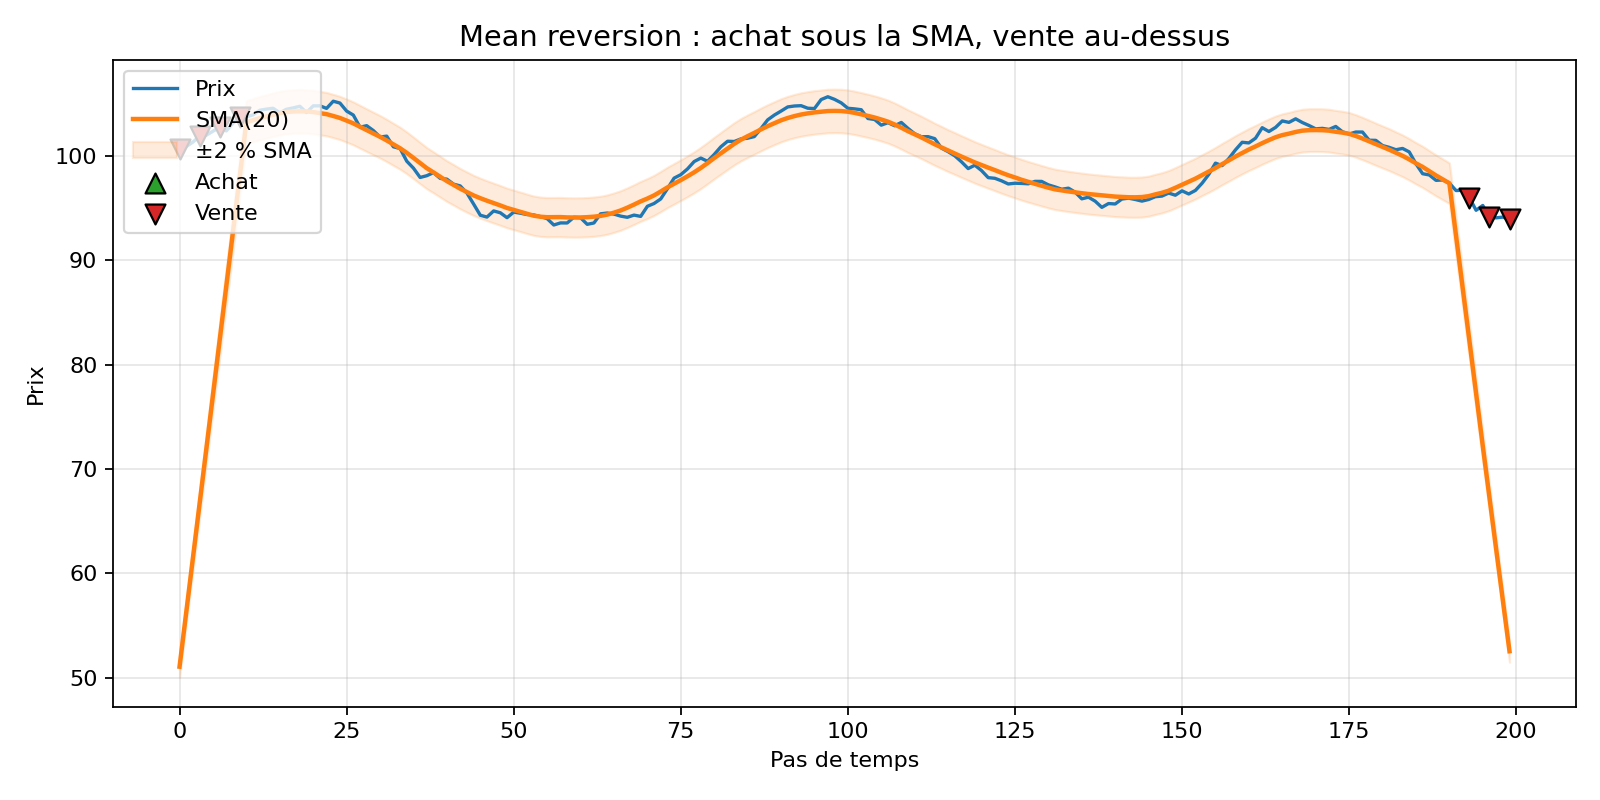
\includegraphics[width=0.78\textwidth]{indic_meanrev.png}

    \vspace{-0.2cm}
    \footnotesize
    \alert{ACHAT} si prix $<$ SMA$-2\%$ \quad $|$ \quad \alert{VENTE} si prix $>$ SMA$+2\%$
\end{frame}

% --- Slide 12 : RSI (visuel)
\begin{frame}{Stratégie : RSI (14)}
    \centering
    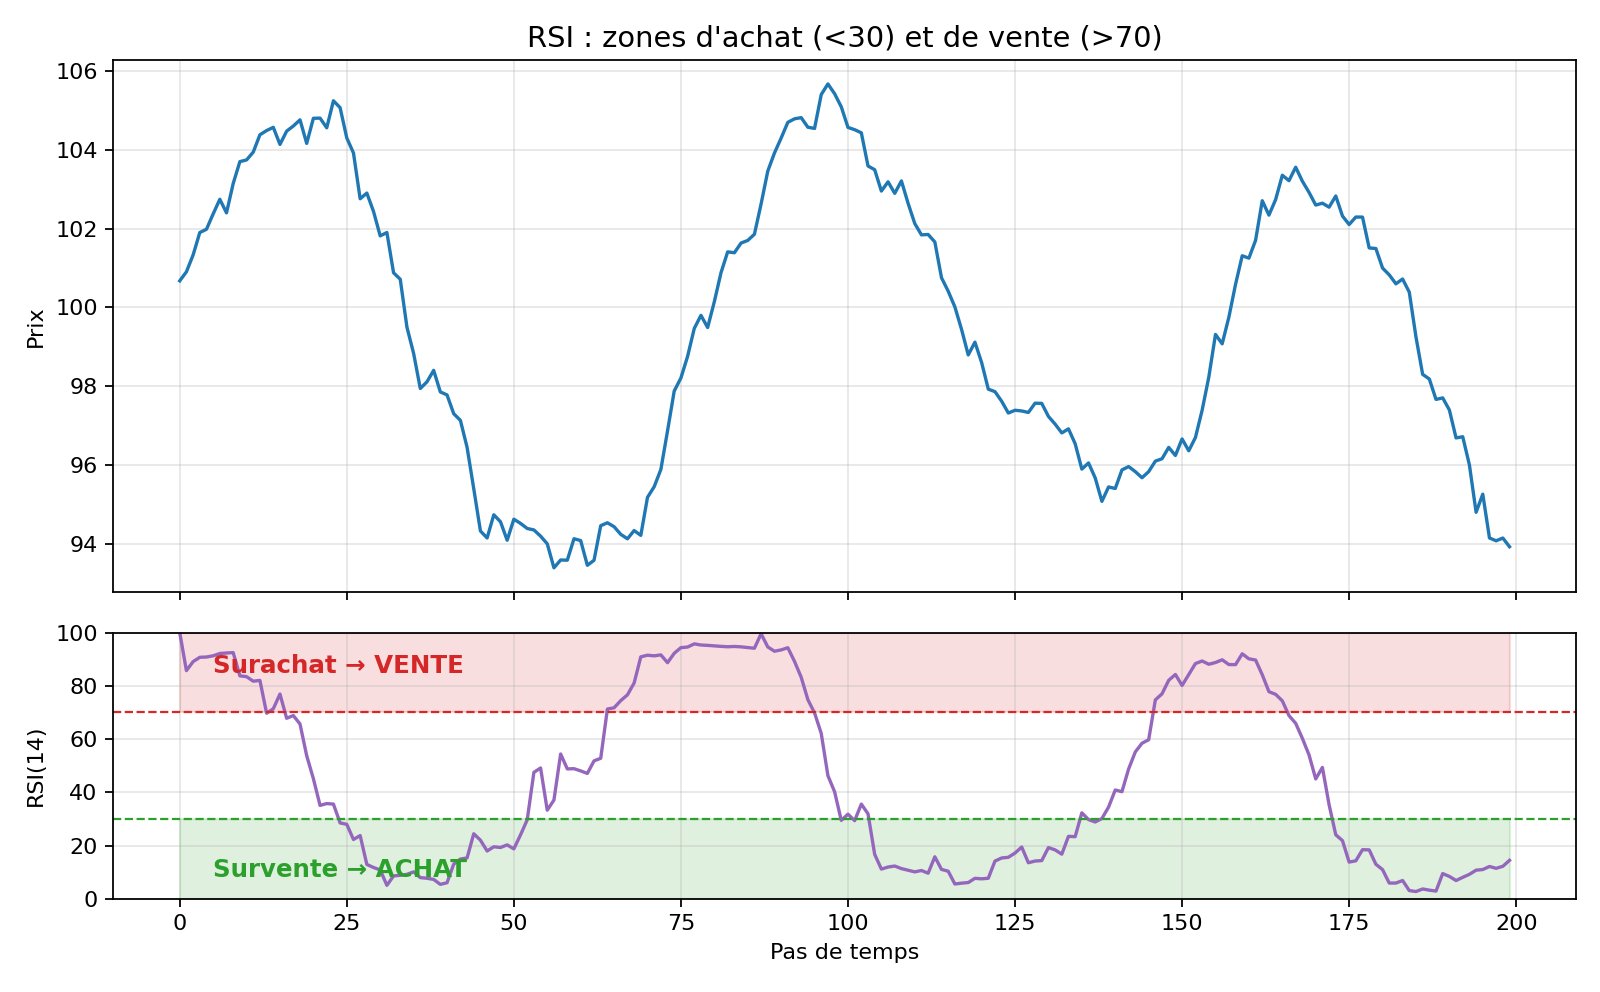
\includegraphics[width=0.7\textwidth]{indic_rsi.png}

    \vspace{-0.1cm}
    \footnotesize
    Oscillateur de momentum : $\text{RSI}<30$ $\rightarrow$ acheter ; $\text{RSI}>70$ $\rightarrow$ vendre.
\end{frame}

% --- Slide 13 : Bollinger (visuel)
\begin{frame}{Stratégie : Bollinger Bands}
    \centering
    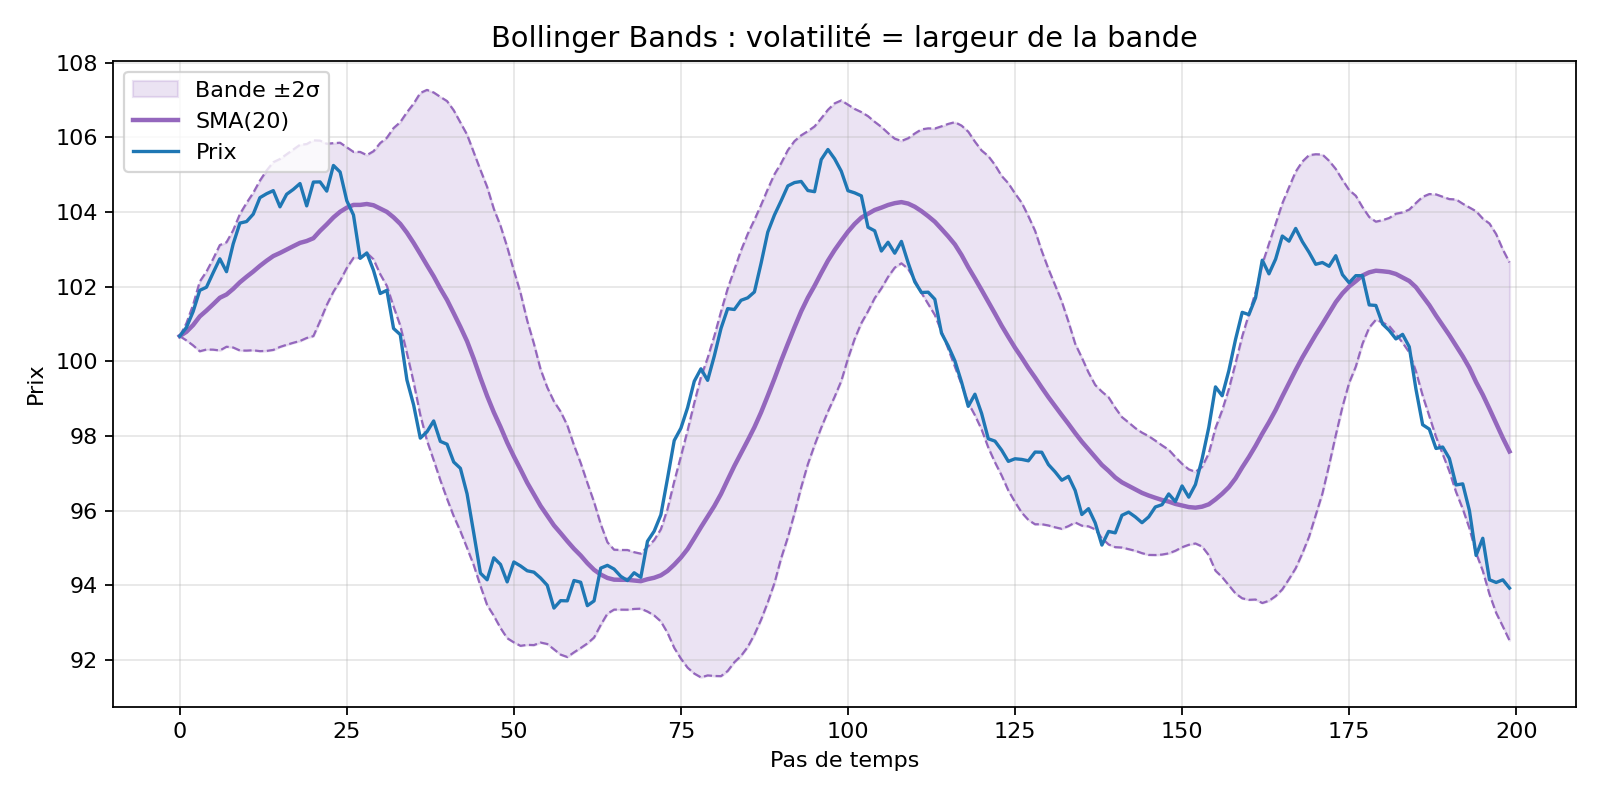
\includegraphics[width=0.78\textwidth]{indic_bollinger.png}

    \vspace{-0.1cm}
    \footnotesize
    Bandes à $\pm 2\sigma$ : largeur $\propto$ volatilité, sortie de bande = signal.
\end{frame}

% --- Slide 14 : Dashboard
\begin{frame}{Tableau de bord}
    \begin{columns}[c]
        \column{0.5\textwidth}
        \centering
        \begin{tikzpicture}[
            every node/.style={font=\tiny},
            screen/.style={draw, rounded corners=2pt, fill=white,
                           minimum width=6cm, minimum height=4cm}
        ]
            \node[screen] (s) {};
            % Header
            \fill[enseirbblue] (s.north west) rectangle ($(s.north east)+(0,-0.4)$);
            \node[white] at ($(s.north)+(0,-0.2)$) {\textbf{Order Book Engine -- Dashboard}};
            % Mini panels
            \node[draw, fill=bidgreen!20, minimum width=2.6cm, minimum height=1.5cm]
                 (p1) at ($(s.north west)+(1.4,-1.3)$) {Carnet};
            \node[draw, fill=enseirbaccent!20, minimum width=2.6cm, minimum height=1.5cm]
                 (p2) at ($(s.north east)+(-1.4,-1.3)$) {Prix + SMA};
            \node[draw, fill=gray!20, minimum width=2.6cm, minimum height=1.2cm]
                 (p3) at ($(s.south west)+(1.4,1.0)$) {PnL / Position};
            \node[draw, fill=yellow!20, minimum width=2.6cm, minimum height=1.2cm]
                 (p4) at ($(s.south east)+(-1.4,1.0)$) {Ordres agent};
        \end{tikzpicture}

        \column{0.5\textwidth}
        \begin{itemize}
            \item Front HTML / CSS / JS
            \item Serveur Python léger
            \item Lecture des JSON :
              \begin{itemize}
                \item \texttt{market\_state.json}
                \item \texttt{agent\_orders.json}
              \end{itemize}
            \item Rafraîchissement périodique
        \end{itemize}
    \end{columns}
\end{frame}

% ===============================================================
% PARTIE 5 -- RL classique
% ===============================================================

% --- Slide 15 : Boucle RL (schéma)
\begin{frame}{Apprentissage par renforcement}
    \centering
    \begin{tikzpicture}[
        every node/.style={font=\footnotesize},
        agent/.style={draw, rounded corners, fill=enseirbblue!20,
                      minimum width=3cm, minimum height=1.4cm, align=center},
        env/.style={draw, rounded corners, fill=enseirbaccent!20,
                    minimum width=3cm, minimum height=1.4cm, align=center},
        arr/.style={->, very thick, >=stealth}
    ]
        \node[agent] (a) at (0,0)   {\textbf{Agent}\\\tiny politique $\pi$};
        \node[env]   (e) at (6,0)   {\textbf{Environnement}\\\tiny carnet d'ordres};

        \draw[arr, enseirbblue]    (a.north) to[bend left=30] node[above]{action $a_t$ \alert{(BUY/SELL/HOLD)}} (e.north);
        \draw[arr, enseirbaccent]  (e.south) to[bend left=30] node[below, align=center]{état $s_t$ \alert{+} récompense $r_t$ \\ \tiny (imbalance, spread, momentum, inventaire, vol)} (a.south);
    \end{tikzpicture}

    \vspace{0.4cm}
    \begin{block}{MDP du trading}
        L'agent observe l'\alert{état}, choisit une \alert{action}, reçoit une \alert{récompense} (variation de PnL pénalisée par l'inventaire).
    \end{block}
\end{frame}

% --- Slide 16 : DQN (architecture visuelle)
\begin{frame}{DQN -- Deep Q-Network}
    \centering
    \begin{tikzpicture}[
        every node/.style={font=\footnotesize},
        layer/.style={draw, rounded corners, minimum width=1.5cm, minimum height=2.5cm, align=center},
        arr/.style={->, thick, >=stealth}
    ]
        \node[layer, fill=enseirbblue!10]  (s)  at (0,0)   {\textbf{État}\\$s_t$\\\tiny dim 6};
        \node[layer, fill=enseirbblue!20]  (h1) at (2,0)   {\textbf{MLP}\\\tiny SiLU\\\tiny LayerNorm};
        \node[layer, fill=enseirbblue!30]  (du) at (4.5,0.9){\textbf{V(s)}};
        \node[layer, fill=enseirbblue!30]  (du2)at (4.5,-0.9){\textbf{A(s,a)}};
        \node[layer, fill=enseirbaccent!25](q)  at (7,0)   {\textbf{Q(s,a)}\\\tiny BUY\\\tiny SELL\\\tiny HOLD};

        \draw[arr] (s) -- (h1);
        \draw[arr] (h1) -- (du);
        \draw[arr] (h1) -- (du2);
        \draw[arr] (du) -- (q);
        \draw[arr] (du2) -- (q);

        \node[font=\scriptsize, enseirbaccent] at (4.5, 2.2) {\textbf{Dueling}};
    \end{tikzpicture}

    \vspace{0.4cm}
    \footnotesize
    \begin{tabular}{ll}
        \alert{Dueling} & $Q(s,a) = V(s) + (A(s,a) - \overline{A})$ \\
        \alert{Double DQN} & cible découplée, anti-surestimation \\
        \alert{Replay buffer} & 200\,k transitions \\
        \alert{Huber loss} + clipping & stabilité numérique \\
    \end{tabular}
\end{frame}

% --- Slide 17 : DQN courbes
\begin{frame}{DQN -- Apprentissage}
    \centering
    \IfFileExists{figures/dqn_training_metrics.png}{%
        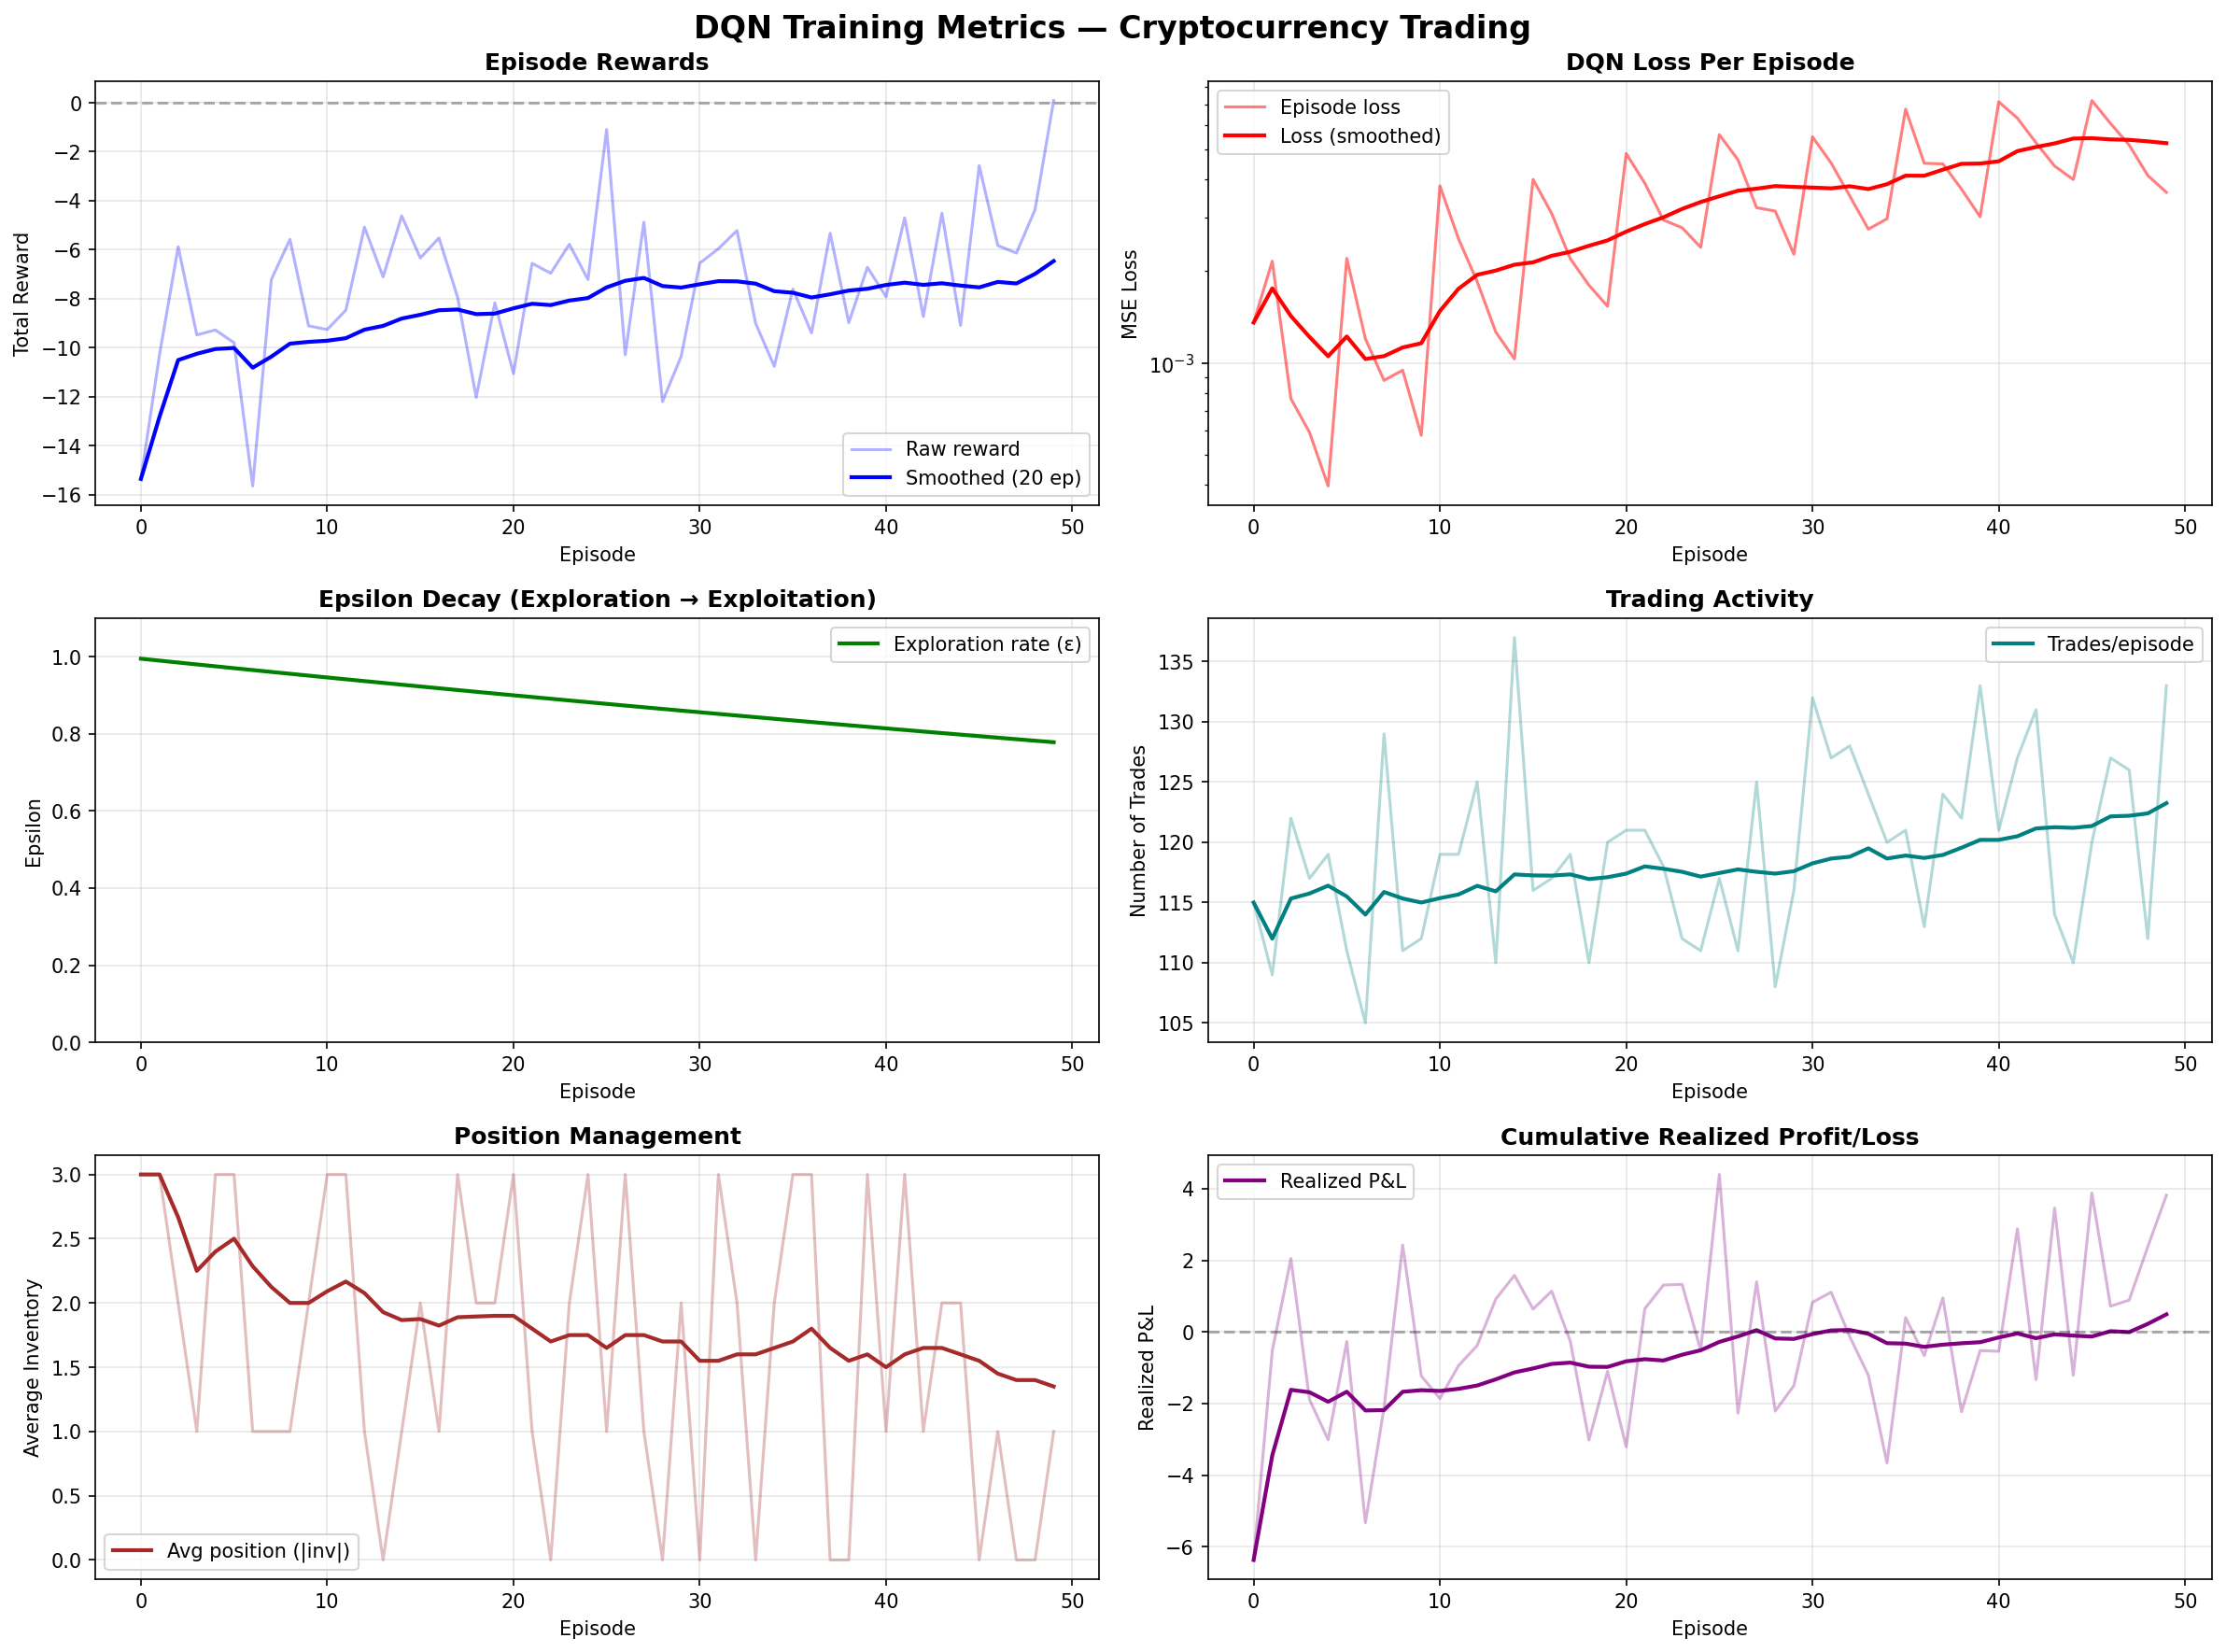
\includegraphics[width=0.9\textwidth,height=0.85\textheight,keepaspectratio]{dqn_training_metrics.png}
    }{%
        \IfFileExists{dqn_training_metrics.png}{%
            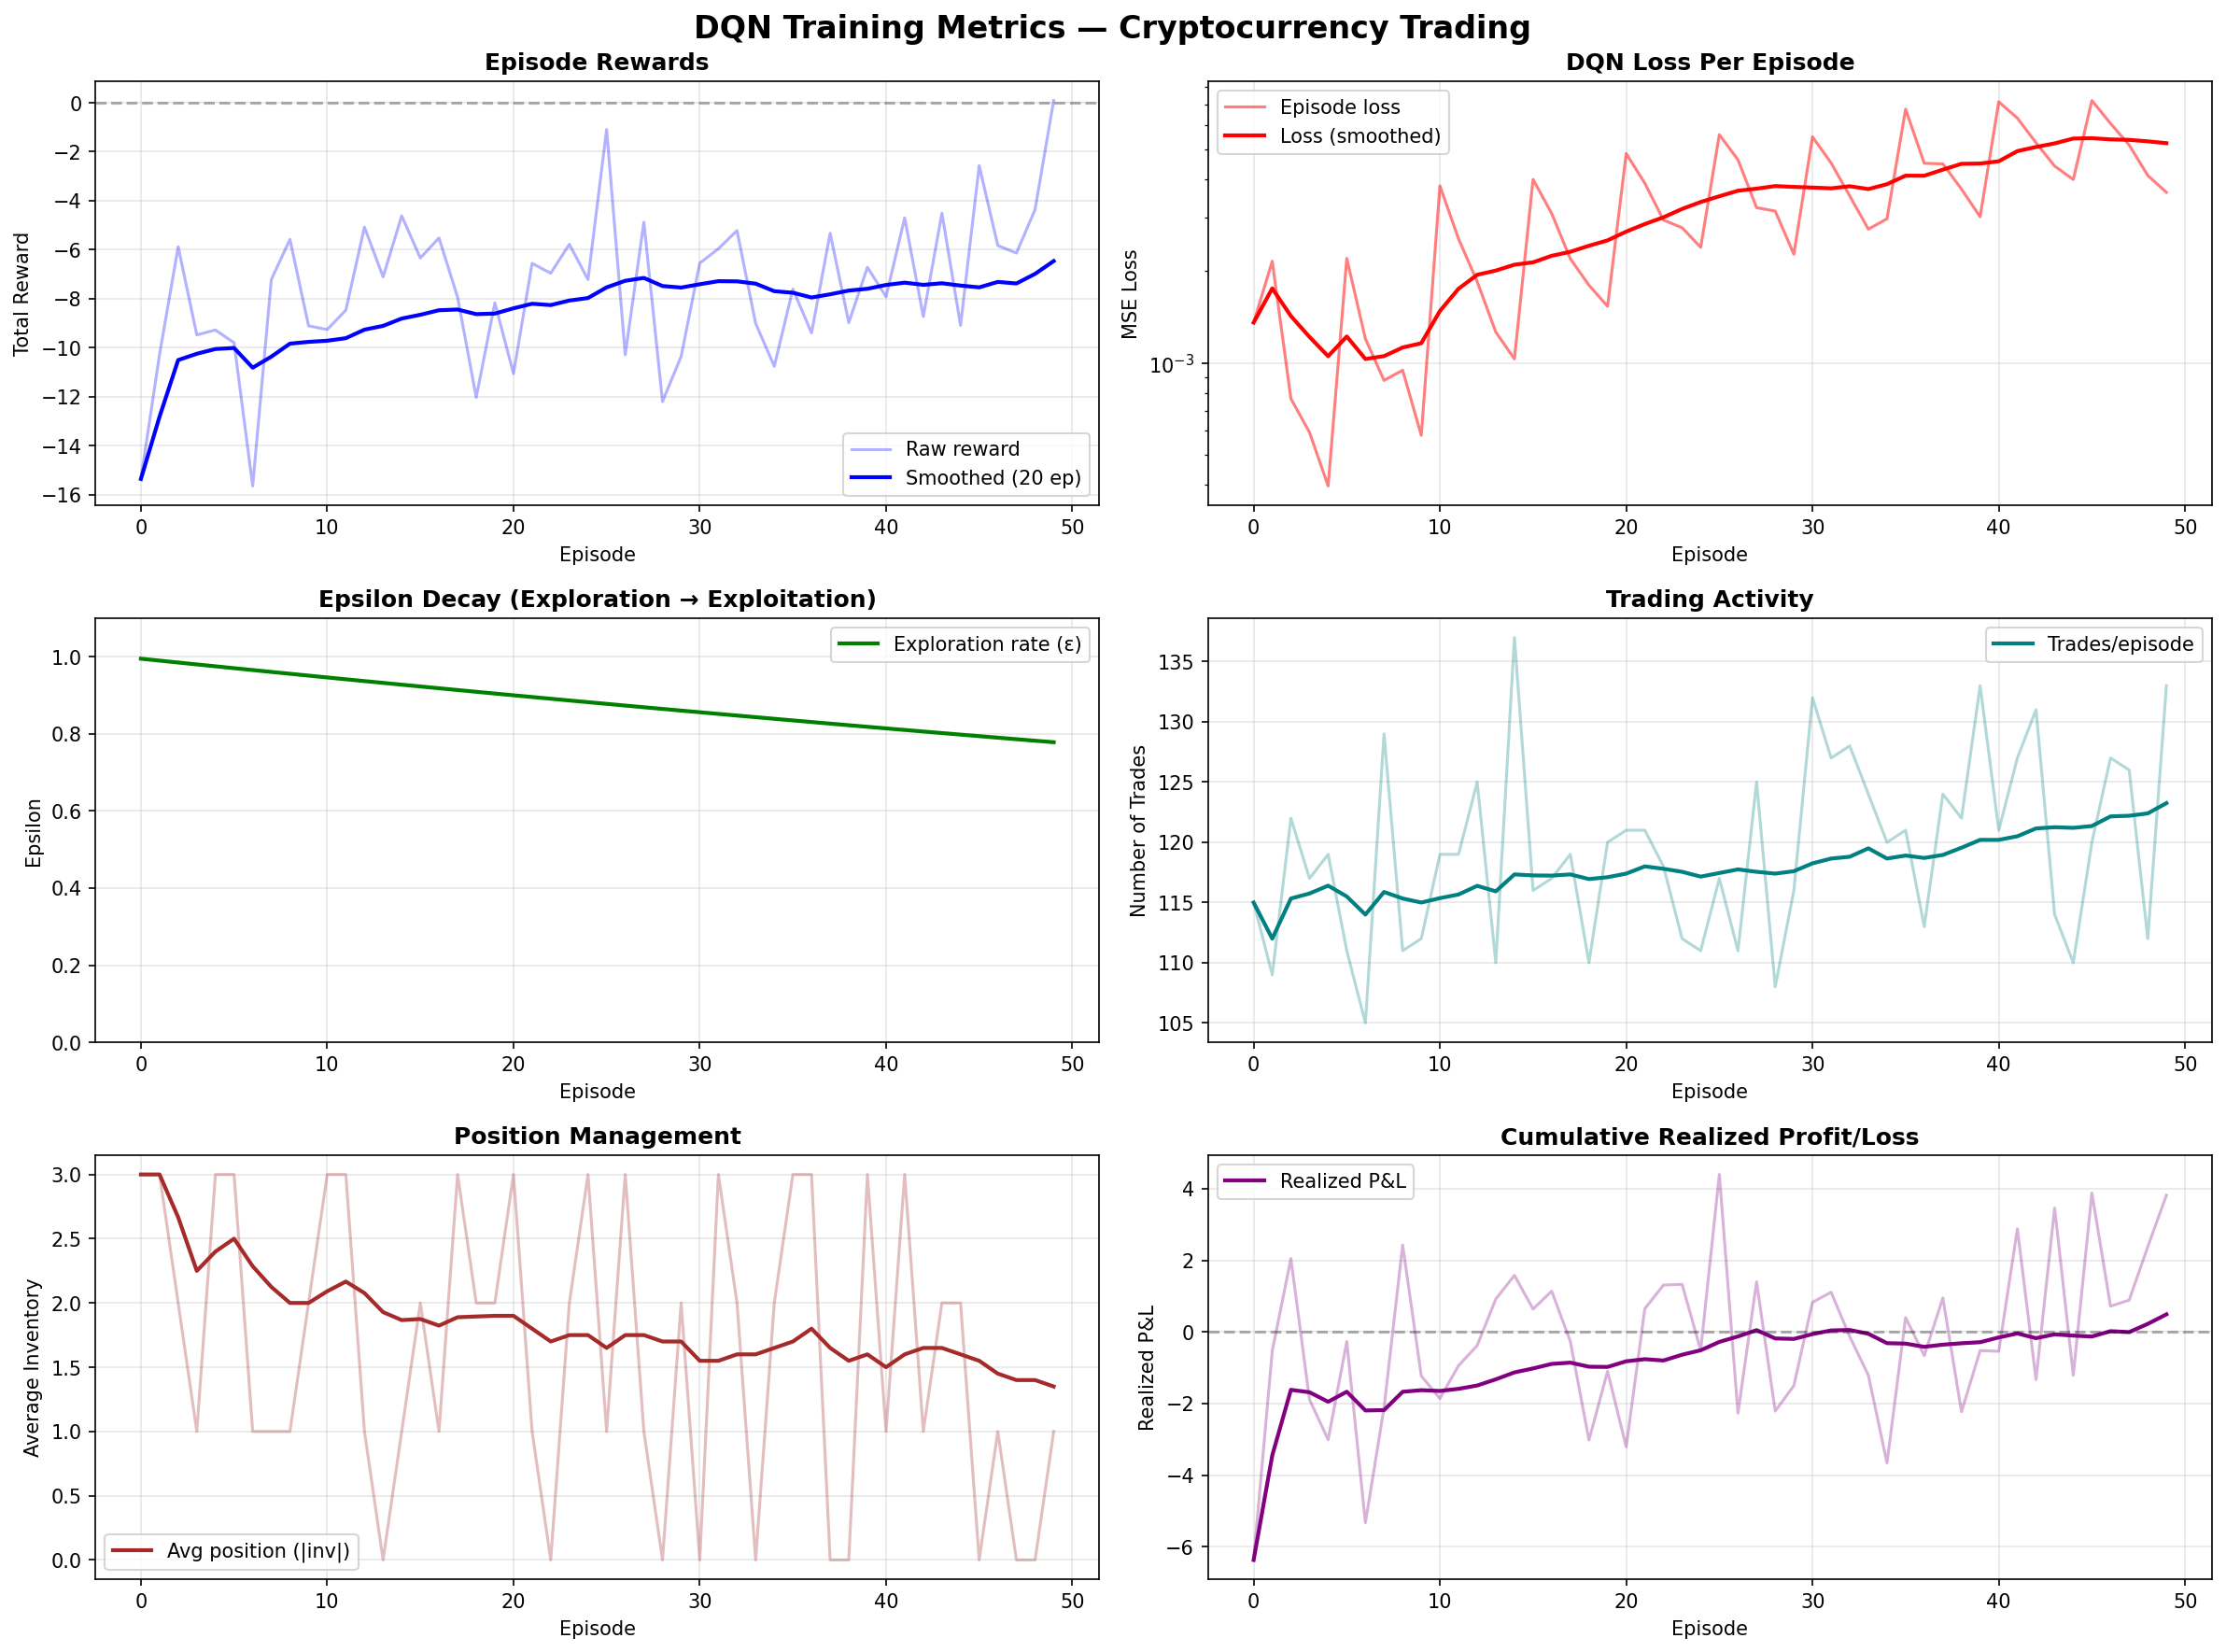
\includegraphics[width=0.9\textwidth,height=0.85\textheight,keepaspectratio]{dqn_training_metrics.png}
        }{%
            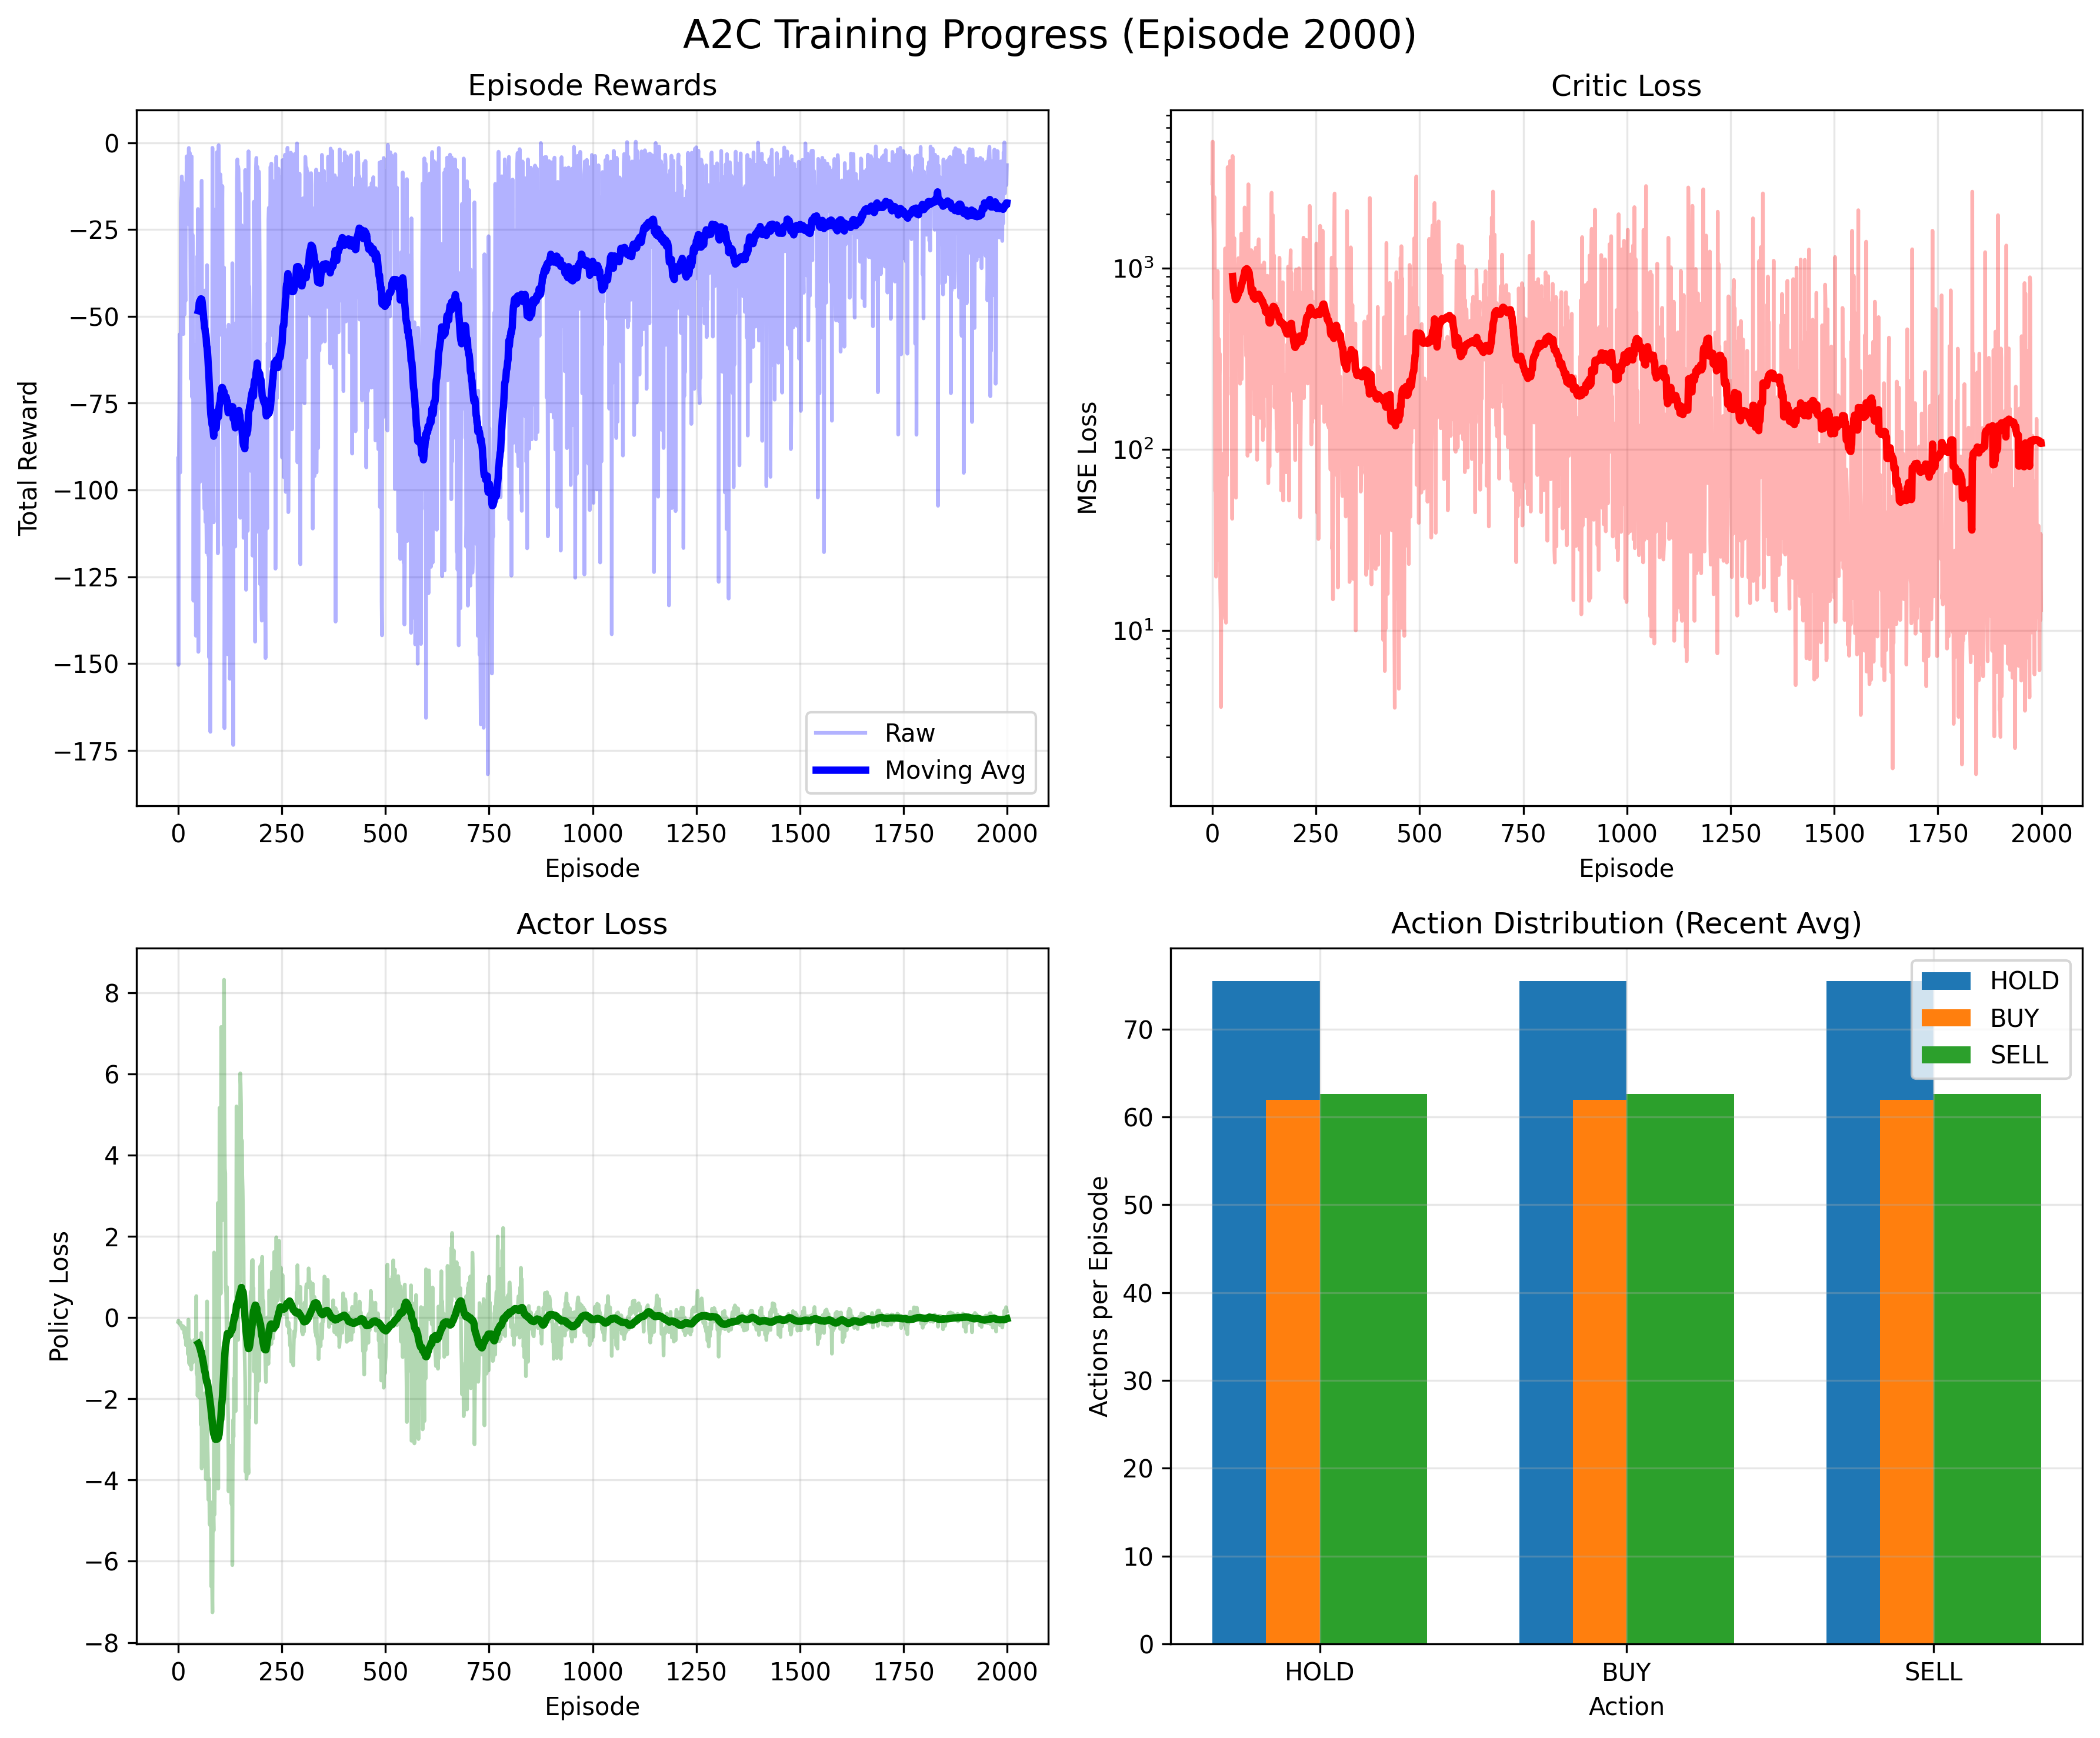
\includegraphics[width=0.9\textwidth,height=0.85\textheight,keepaspectratio]{a2c_training_metrics.png}
        }
    }
\end{frame}

% --- Slide 18 : Actor-Critic (schéma)
\begin{frame}{A2C -- Actor-Critic}
    \centering
    \begin{tikzpicture}[
        every node/.style={font=\footnotesize},
        box/.style={draw, rounded corners, minimum width=2cm, minimum height=1cm, align=center},
        arr/.style={->, thick, >=stealth}
    ]
        \node[box, fill=gray!20] (s) at (0,0) {État $s$};
        \node[box, fill=enseirbblue!25] (trunk) at (3,0) {Tronc partagé};
        \node[box, fill=enseirbaccent!25] (actor)  at (6.5,1)  {\textbf{Acteur}\\\tiny$\pi(a|s)$};
        \node[box, fill=bidgreen!25]      (critic) at (6.5,-1) {\textbf{Critique}\\\tiny$V(s)$};

        \draw[arr] (s) -- (trunk);
        \draw[arr] (trunk) -- (actor);
        \draw[arr] (trunk) -- (critic);

        \node[font=\tiny] at (9,1)  {action $a_t$};
        \node[font=\tiny] at (9,-1) {valeur $V_t$};
        \draw[arr] (actor)  -- (9,1);
        \draw[arr] (critic) -- (9,-1);
    \end{tikzpicture}

    \vspace{0.3cm}
    \footnotesize
    \begin{tabular}{ll}
        \alert{Avantage} & $A_t = R_t - V(s_t)$ \\
        $\mathcal{L}_{\text{actor}}$  & $-\log \pi(a_t|s_t)\, A_t$ \\
        $\mathcal{L}_{\text{critic}}$ & $(R_t - V(s_t))^2$ \\
    \end{tabular}
\end{frame}

% --- Slide 19 : A2C courbes
\begin{frame}{A2C -- Apprentissage}
    \centering
    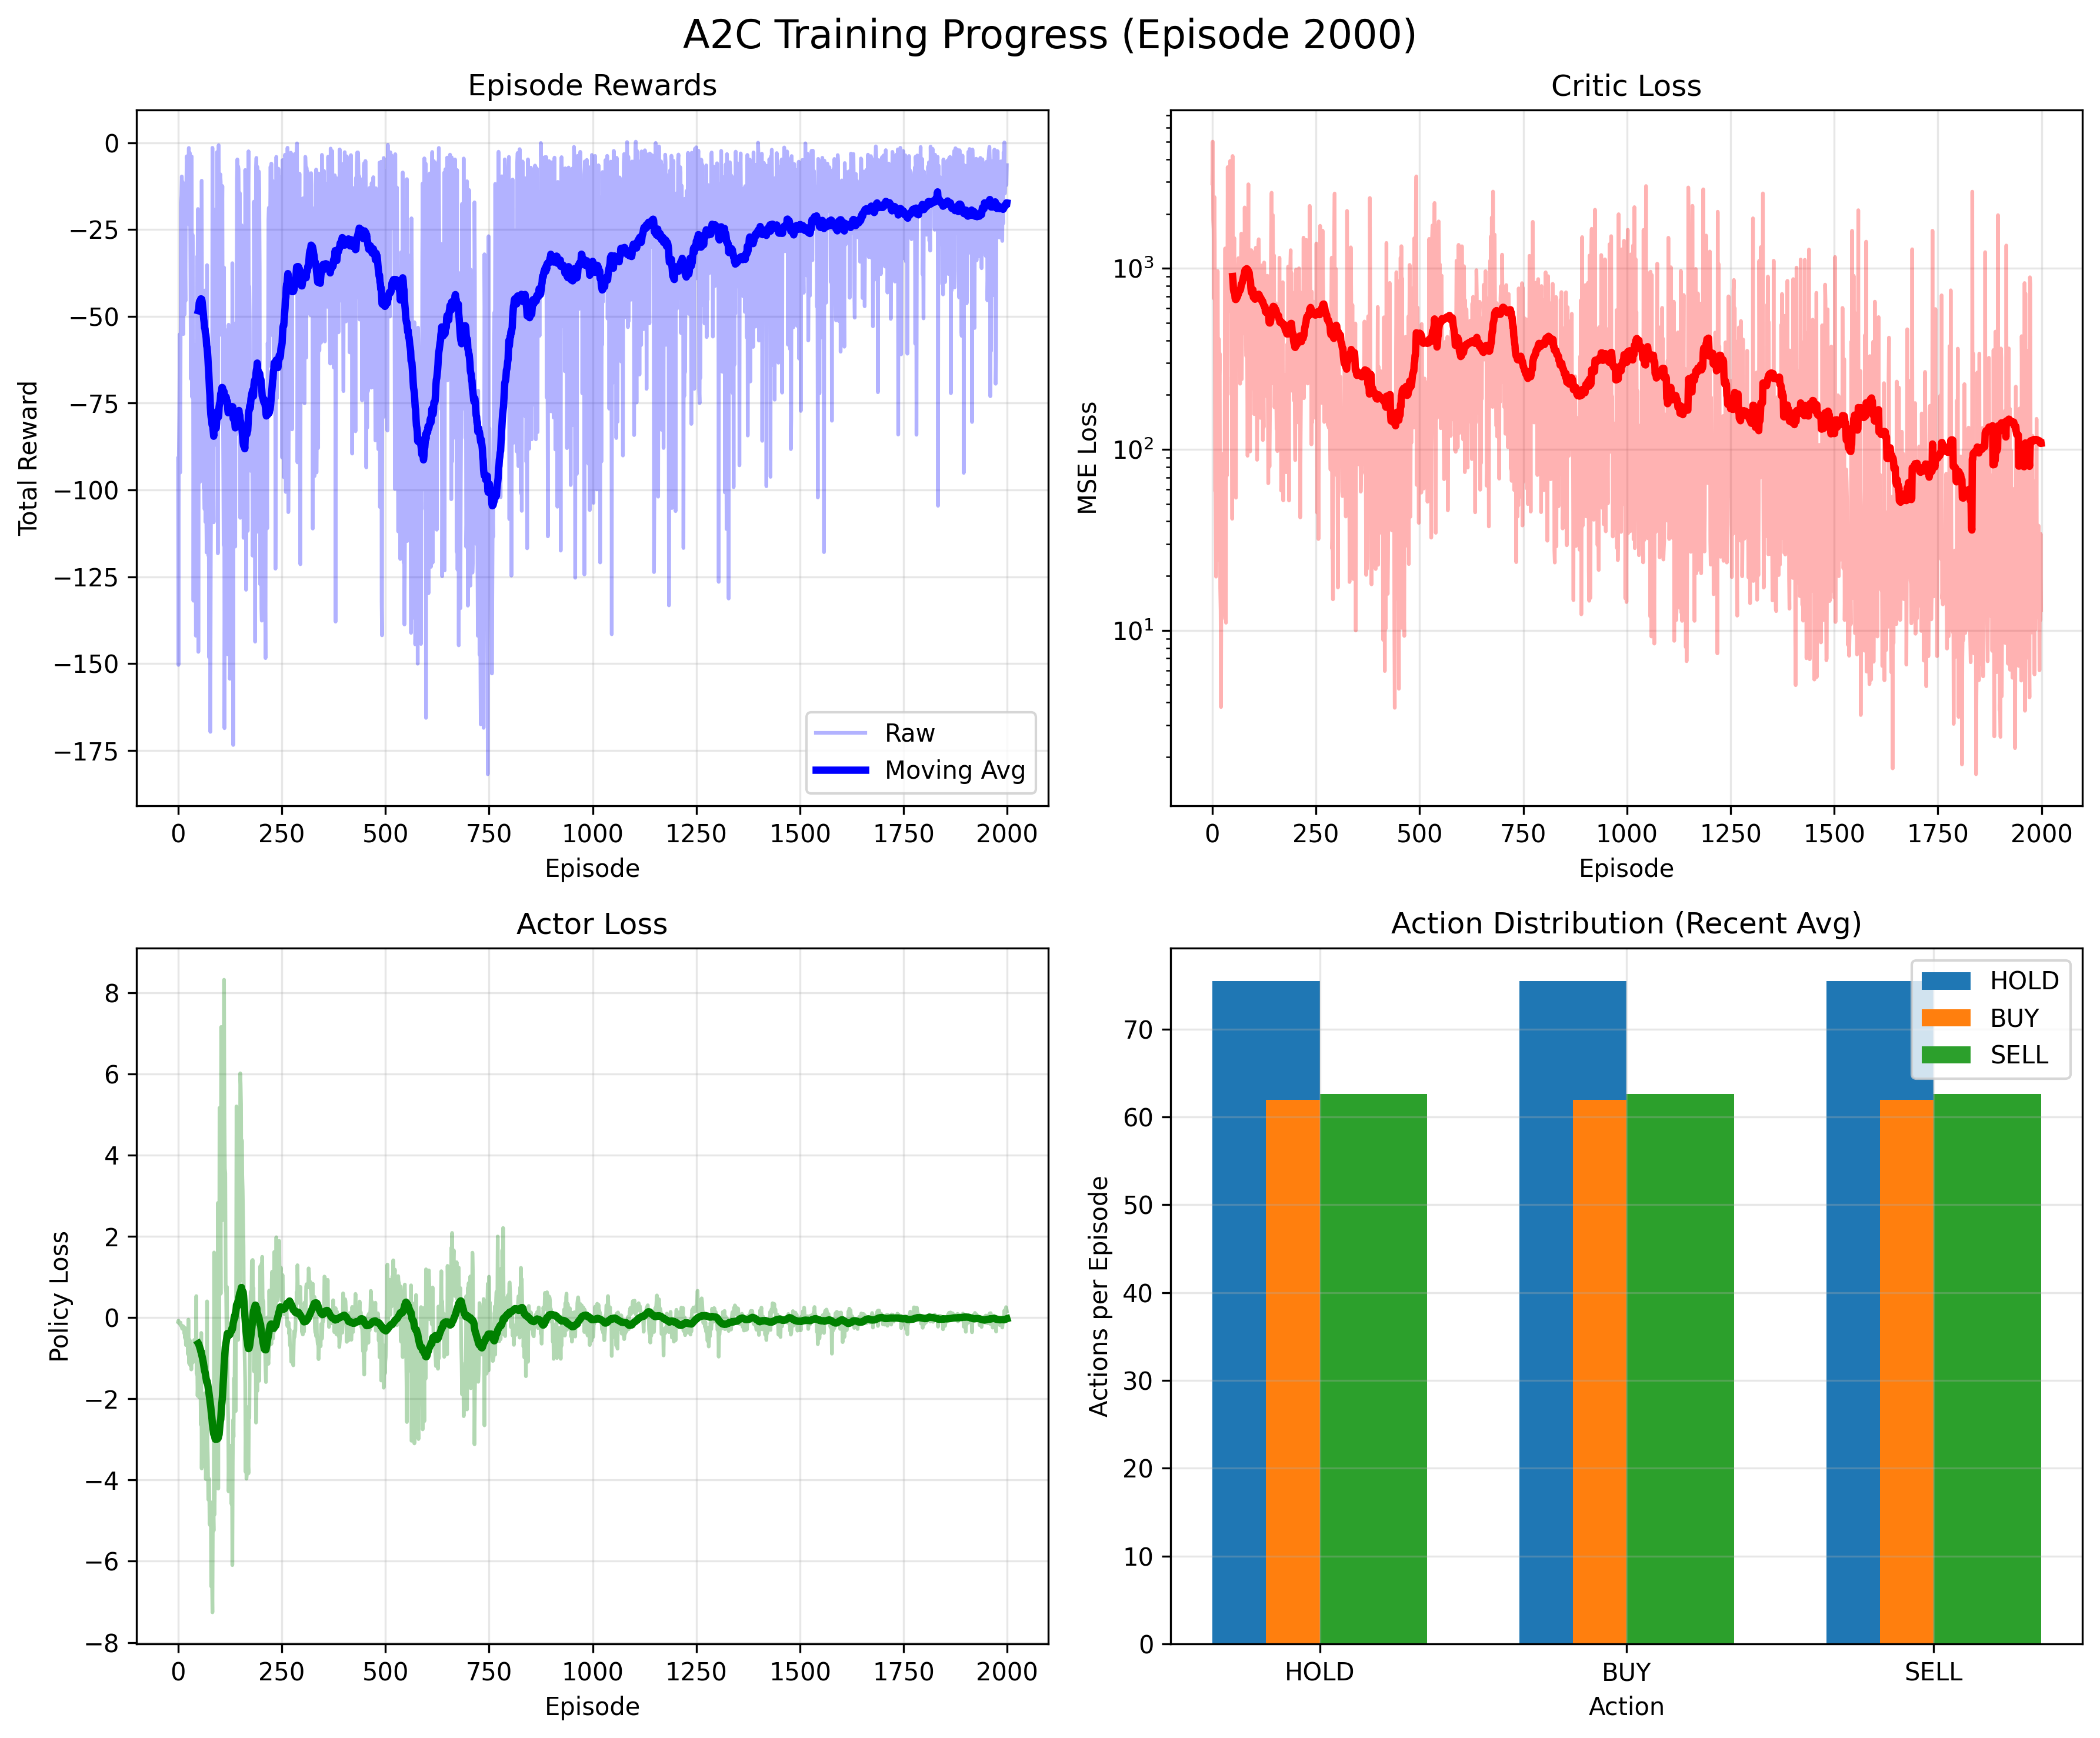
\includegraphics[width=0.9\textwidth,height=0.85\textheight,keepaspectratio]{a2c_training_metrics.png}
\end{frame}

% --- Slide 20 : PPO
\begin{frame}{PPO -- Proximal Policy Optimization}
    \begin{block}{Idée : limiter l'écart entre la nouvelle politique et l'ancienne}
        \[
        \mathcal{L}^{\text{CLIP}} = \mathbb{E}_t\!\left[
            \min\!\big(r_t A_t,\;
            \mathrm{clip}(r_t, 1-\epsilon, 1+\epsilon)\, A_t\big)
        \right]
        \]
    \end{block}

    \centering
    \begin{tikzpicture}[
        every node/.style={font=\scriptsize}
    ]
        \draw[->] (-0.5,0) -- (5,0) node[right]{$r_t$};
        \draw[->] (0,-0.5) -- (0,1.5) node[above]{clip};
        \draw[red, thick] (0,0) -- (1,1) -- (3,1) -- (4.5,1.45);
        \draw[gray, dashed] (1,0) -- (1,1);
        \draw[gray, dashed] (3,0) -- (3,1);
        \node at (1,-0.3) {$1-\epsilon$};
        \node at (3,-0.3) {$1+\epsilon$};
        \node[red] at (4,1.65) {sans clip};
        \node[red] at (2,1.3) {clipé};
    \end{tikzpicture}

    \vspace{0.1cm}
    \footnotesize
    \alert{Plus stable que A2C} : pas de divergence brutale, plusieurs époques par batch.
\end{frame}

% --- Slide 21 : PPO courbes
\begin{frame}{PPO -- Apprentissage}
    \centering
    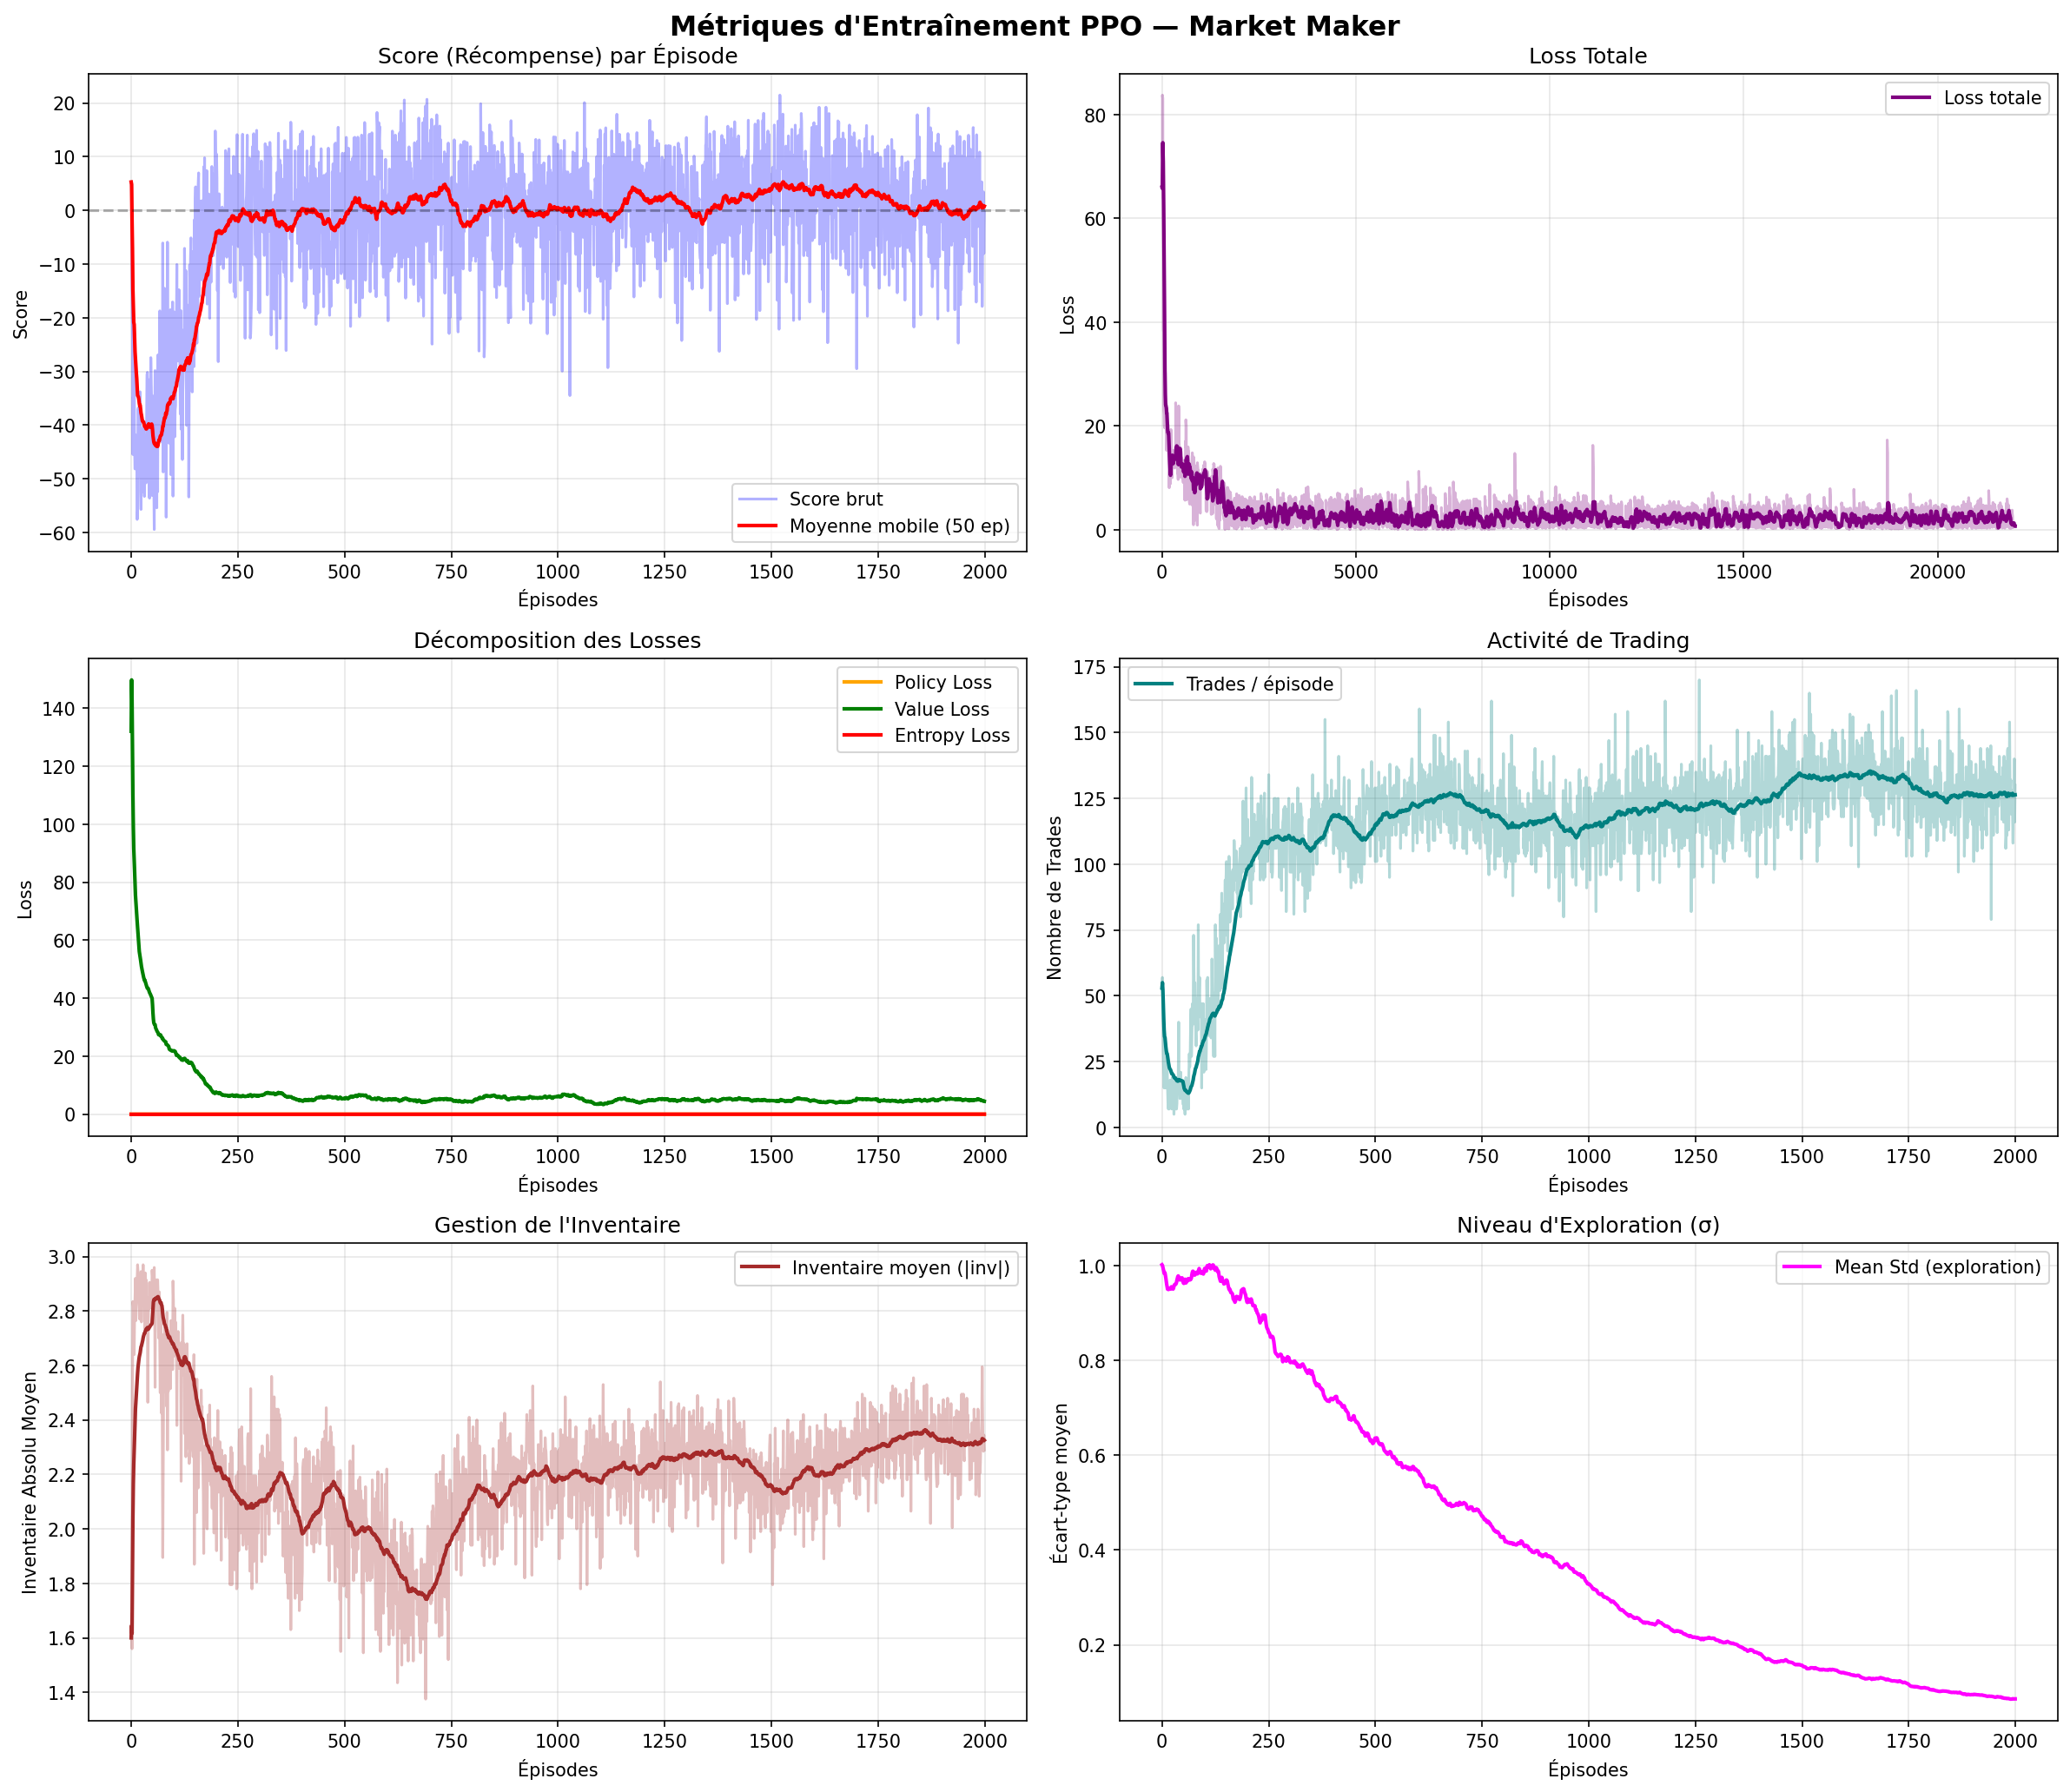
\includegraphics[width=0.9\textwidth,height=0.85\textheight,keepaspectratio]{courbe_apprentissage.png}
\end{frame}

% ===============================================================
% PARTIE 6 -- Dreamer + conclusion
% ===============================================================

% --- Slide 22 : Dreamer principe
\begin{frame}{Dreamer v3 -- Apprendre dans l'imagination}
    \centering
    \begin{tikzpicture}[
        every node/.style={font=\footnotesize},
        env/.style={draw, rounded corners, fill=gray!20,
                    minimum width=2.5cm, minimum height=1cm, align=center},
        wm/.style={draw, rounded corners, fill=enseirbaccent!20,
                   minimum width=2.5cm, minimum height=1cm, align=center},
        ag/.style={draw, rounded corners, fill=enseirbblue!20,
                   minimum width=2.5cm, minimum height=1cm, align=center},
        arr/.style={->, thick, >=stealth}
    ]
        \node[env] (env) at (0,0) {\textbf{Environnement} \\ \tiny réel};
        \node[wm]  (wm)  at (4,0) {\textbf{World Model} \\ \tiny RSSM};
        \node[ag]  (ac)  at (8,0) {\textbf{Acteur--Critique}};

        \draw[arr] (env) -- node[above]{\tiny obs / récompense} (wm);
        \draw[arr] (wm.north east) to[bend left=25] node[above]{\tiny rollouts imaginés}  (ac.north west);
        \draw[arr] (ac.south west) to[bend left=25] node[below]{\tiny actions}  (wm.south east);
    \end{tikzpicture}

    \vspace{0.4cm}
    \begin{block}{Idée clé}
        Apprendre la dynamique du marché dans un \alert{World Model},
        puis entraîner l'acteur sur des trajectoires imaginées --- \emph{sans} interagir avec l'environnement réel.
    \end{block}
\end{frame}

% --- Slide 23 : Dreamer RSSM zoom
\begin{frame}{Dreamer v3 -- World Model (RSSM)}
    \centering
    \begin{tikzpicture}[
        every node/.style={font=\scriptsize},
        node distance=1cm,
        circ/.style={draw, circle, minimum size=0.85cm, fill=enseirbblue!15},
        sq/.style={draw, rounded corners, minimum width=0.95cm, minimum height=0.7cm, fill=enseirbaccent!15},
        arr/.style={->, >=stealth}
    ]
        \node[circ] (h0) at (0,0) {$h_{t-1}$};
        \node[circ] (h1) at (3,0) {$h_t$};
        \node[circ] (h2) at (6,0) {$h_{t+1}$};

        \node[sq, above=of h1] (z1) {$z_t$};
        \node[sq, above=of h2] (z2) {$z_{t+1}$};

        \node[sq, below=of h1, fill=gray!20] (x1) {$x_t$};
        \node[sq, below=of h2, fill=gray!20] (x2) {$x_{t+1}$};

        \draw[arr] (h0) -- node[above]{\tiny GRU} (h1);
        \draw[arr] (h1) -- node[above]{\tiny GRU} (h2);
        \draw[arr] (h1) -- (z1);
        \draw[arr] (h2) -- (z2);
        \draw[arr] (x1) -- (h1);
        \draw[arr] (x2) -- (h2);
    \end{tikzpicture}

    \vspace{0.3cm}
    \footnotesize
    \alert{Latents catégoriels $32\times32$} \;|\;
    \alert{GRU} récurrent \;|\;
    \alert{symlog} pour stabilité numérique
\end{frame}

% --- Slide 24 : Dreamer courbes
\begin{frame}{Dreamer v3 -- Apprentissage}
    \centering
    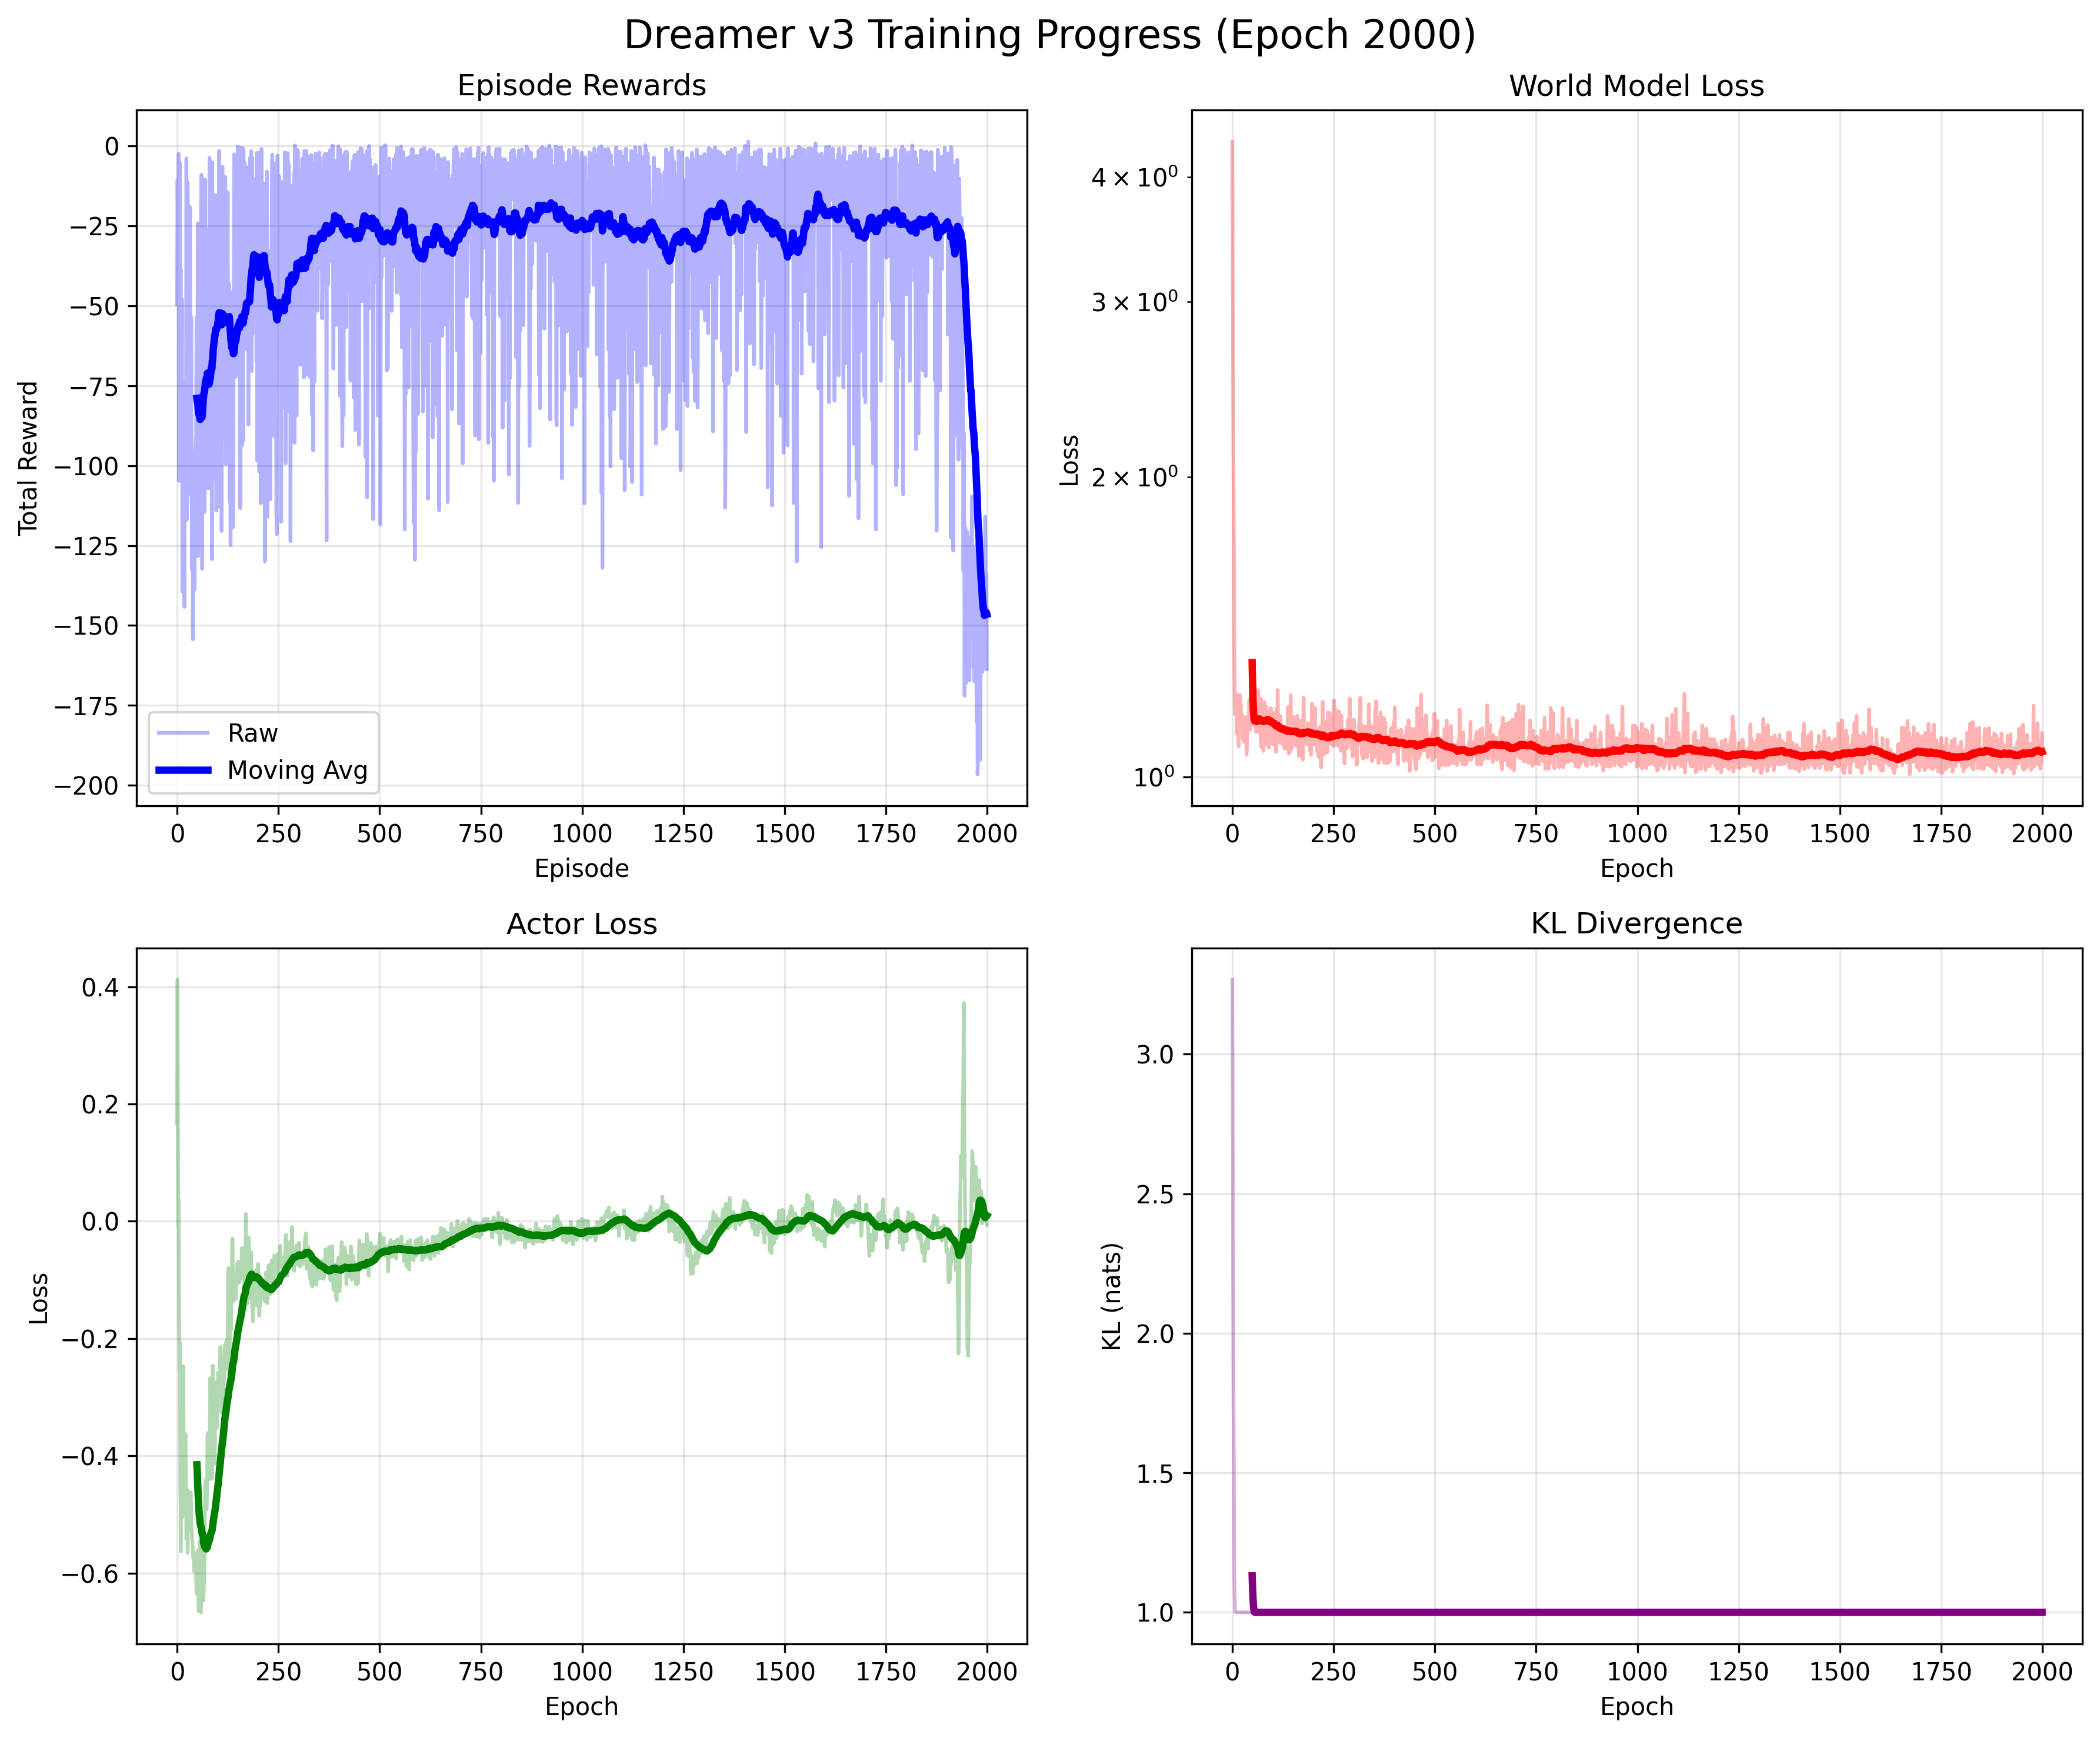
\includegraphics[width=0.9\textwidth,height=0.85\textheight,keepaspectratio]{dreamer_training_metrics.png}
\end{frame}

% --- Slide 25a : Protocole de backtest
\begin{frame}{Comparaison -- Protocole de test}
    \begin{columns}[T]
        \column{0.5\textwidth}
        \textbf{\color{enseirbblue}Données}
        \begin{itemize}
            \item Source : \alert{Binance aggTrades}
            \item Symbole : \texttt{SOLUSDT}
            \item Période : \alert{février 2026}
            \item $\sim 6$ millions de trades agrégés
            \item Régime : tendance baissière $105 \to 85$ USDT
        \end{itemize}

        \column{0.5\textwidth}
        \textbf{\color{enseirbblue}Backtest}
        \begin{itemize}
            \item \alert{6000 bougies} de 1000 ticks
            \item Quantité : 1 SOL / ordre
            \item Inventaire : $\pm 5$ positions max
            \item PnL \alert{mark-to-market}
            \item Sharpe annualisé, drawdown max
            \item \texttt{seed = 42} (reproductible)
        \end{itemize}
    \end{columns}

    \vspace{0.3cm}
    \begin{block}{Conditions communes}
        Toutes les stratégies (règles \emph{et} RL) sont évaluées sur \alert{le même flux de prix},
        avec la même fonction de coût et les mêmes bornes d'inventaire.
        Seule la politique de décision change.
    \end{block}
\end{frame}

% --- Slide 25b : Tableau de résultats
\begin{frame}{Comparaison -- Résultats}
    \IfFileExists{comparison_table.tex}{% Tableau généré automatiquement par agents/compute_metrics.py
% Backtest sur SOLUSDT-aggTrades-2026-02 (6000 bougies, 1000 trades/bougie)
\begin{center}
\scriptsize
\begin{tabularx}{\textwidth}{lrrrX}
    \toprule
    \textbf{Stratégie} & \textbf{PnL final (USDT)} & \textbf{Sharpe} & \textbf{Drawdown max} & \textbf{Remarques} \\
    \midrule
    Mean Reversion & +56.62 & 0.14 & -82.56 & baseline règles \\
    RSI & +6.08 & 0.01 & -101.69 & baseline règles \\
    Bollinger & -108.09 & -0.28 & -157.04 & baseline règles \\
    DQN & +78.92 & 0.18 & -99.77 & value-based \\
    A2C & +27.05 & 0.06 & -129.23 & policy-based \\
    PPO & +42.07 & 0.10 & -117.47 & policy-based stable \\
    Dreamer v3 & +49.27 & 0.13 & -61.43 & model-based \\
    \bottomrule
\end{tabularx}
\end{center}
}{% Tableau généré automatiquement par agents/compute_metrics.py
% Backtest sur SOLUSDT-aggTrades-2026-02 (6000 bougies, 1000 trades/bougie)
\begin{center}
\scriptsize
\begin{tabularx}{\textwidth}{lrrrX}
    \toprule
    \textbf{Stratégie} & \textbf{PnL final (USDT)} & \textbf{Sharpe} & \textbf{Drawdown max} & \textbf{Remarques} \\
    \midrule
    Mean Reversion & +56.62 & 0.14 & -82.56 & baseline règles \\
    RSI & +6.08 & 0.01 & -101.69 & baseline règles \\
    Bollinger & -108.09 & -0.28 & -157.04 & baseline règles \\
    DQN & +78.92 & 0.18 & -99.77 & value-based \\
    A2C & +27.05 & 0.06 & -129.23 & policy-based \\
    PPO & +42.07 & 0.10 & -117.47 & policy-based stable \\
    Dreamer v3 & +49.27 & 0.13 & -61.43 & model-based \\
    \bottomrule
\end{tabularx}
\end{center}
}

    \vspace{0.2cm}
    \footnotesize
    \begin{itemize}
        \item \alert{DQN} et \alert{Dreamer v3} dominent en PnL.
        \item Dreamer affiche le meilleur \alert{drawdown} (inertie d'action).
        \item Bollinger souffre de la baisse soutenue $105 \to 85$ USDT.
    \end{itemize}
\end{frame}

% --- Slide 26 : Conclusion
\begin{frame}{Bilan \& perspectives}
    \begin{columns}[T]
        \column{0.5\textwidth}
        \textbf{\color{bidgreen}Réalisé}
        \begin{itemize}
            \item Moteur C++ $\sim 400$\,k ops/s
            \item Ingestion live Binance
            \item Dashboard interactif
            \item 3 stratégies par règles
            \item 4 agents RL (DQN, A2C, PPO, Dreamer)
        \end{itemize}

        \column{0.5\textwidth}
        \textbf{\color{enseirbaccent}Perspectives}
        \begin{itemize}
            \item Carnet \alert{multi-niveaux}
            \item \emph{Order flow imbalance}
            \item Reward Sharpe-différentiel
            \item \emph{Walk-forward validation}
        \end{itemize}
    \end{columns}

    \vspace{0.6cm}
    \begin{center}
        \Large \alert{Merci de votre attention --- Questions ?}
    \end{center}
\end{frame}

\end{document}
